% Chapter Template

\chapter{Diseño e Implementación} % Main chapter title
% cSpell:words resizebox \textit{onosapi} usecase Mcast enrutamiento parencite includegraphics pcktprocactiv lstlisting iperf

\label{Chapter4} % Change X to a consecutive number; for referencing this chapter elsewhere, use 
% \ref{ChapterX} 
Para el desarrollo del proyecto será necesario implementar un sistema donde se puedan realizar pruebas y evaluar la correctitud del mismo. 

De esta forma, la primera sección de este capítulo comprende tanto el análisis del sistema, como la topología utilizada. Específicamente, se estudiará su estructura, su comportamiento y sus requerimientos. 

En las secciones siguientes, se detallarán las aplicaciones desarrolladas que permiten cumplir con el objetivo del proyecto. En primer lugar, se hará un estudio del módulo \textit{YANG} implementado, el cual caracteriza y modela los datos del equipo. A continuación, se detallará el \textit{driver} implementado para lograr la comunicación entre el controlador y el dispositivo. Por último, se analizará la interfaz \textit{REST} y la \textit{GUI} desarrollada.

%----------------------------------------------------------------------------------------
%	SECTION 1
%----------------------------------------------------------------------------------------

\section{Entorno de trabajo}
En esta sección se detallan las características del sistema a implementar, descriptas en el lenguaje de especificación de sistemas SysML \parencite{sysml}. Se optó por este lenguaje de modelado ya que brinda una extensión a UML permitiendo combinar elementos del mundo físico (\textit{hardware}) con elementos del mundo lógico (\textit{software}). 

%-----------------------------------
%	SUBSECTION 1
%-----------------------------------

\subsection{Topología}

Se conformará una topología con el fin de poder identificar en una primera instancia, los requerimientos que debe cumplir el sistema. La misma, está basada en un caso de uso simple, en el cual se quiere brindar conectividad a dos clientes a través de un enlace óptico, este último conformado por dos \textit{muxponders}.  

Es importante identificar la presencia del controlador \textit{ONOS}, el cual gestionará la configuración de los equipos mediante el protocolo \textit{NETCONF}. En la figura \ref{fig:topologia} se muestra de forma general la topología planteada.

\begin{figure}[H]
    \centering
    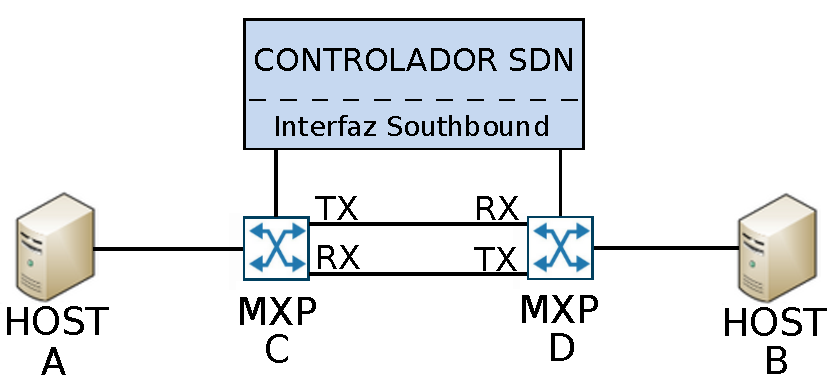
\includegraphics[scale=0.85]{Figures/topologia.pdf}
    \caption{Topología implementada en el proyecto.}
    \label{fig:topologia}
  \end{figure}


Los dispositivos terminales A y B, se encuentran conectados al puerto cliente del \textit{muxponder} C y D, respectivamente. A su vez, el transmisor del \textit{muxponder} C se encuentra conectado con el receptor del \textit{muxponder} D, y viceversa. Esto permite una comunicación bidireccional, donde ambos clientes pueden tener conectividad. 

Por otra parte, el controlador tiene una conexión con los \textit{muxponder} a través de los puertos de control de los mismos.

\begin{comment}
A continuación, en la figura \ref{fig:topologiafis} se muestra como está dispuesta la conexión físicamente en los dispositivos. A la izquierda se tiene el \textit{muxponder} C, y a la derecha se encuentra el \textit{muxponder} D. Las interfaces de control de ambos dispositivos están conectadas al controlador \textit{ONOS}, mientras que los puertos clientes se encuentran conectados a los clientes A y B respectivamente. Por otra parte, las interfaces de línea se encuentran conectados entre los \textit{muxponder}, como se explicó anteriormente, con el fin de poder tener una comunicación bidireccional.
\end{comment}

\begin{comment}
\begin{figure}[H]
    \centering
    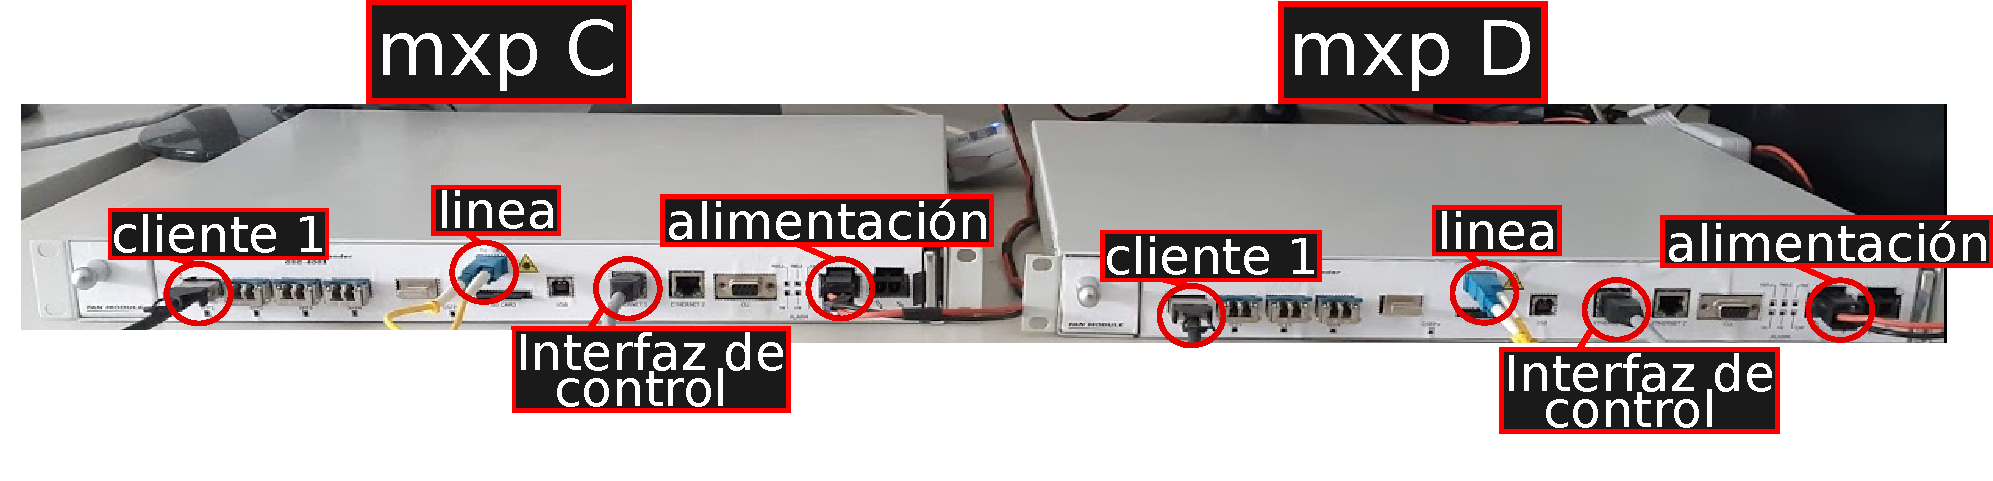
\includegraphics[scale=0.45]{Figures/mxpfisicos.pdf}
    \caption{Conexión física de la topología.}
    \label{fig:topologiafis}
  \end{figure}
\end{comment}

%-----------------------------------
%	SUBSECTION 2
%-----------------------------------
\subsection{Requerimientos del sistema}

Para establecer los requerimientos funcionales del sistema, se presentará en primer lugar un diagrama de caso de uso. Como se puede observar en la figura \ref{fig:caso_uso_admin}, el objeto principal del sistema es poder brindar al administrador un entorno donde pueda gestionar la configuración de los \textit{muxponders} mediante sus aplicaciones.

\begin{figure}[H]
    \centering
    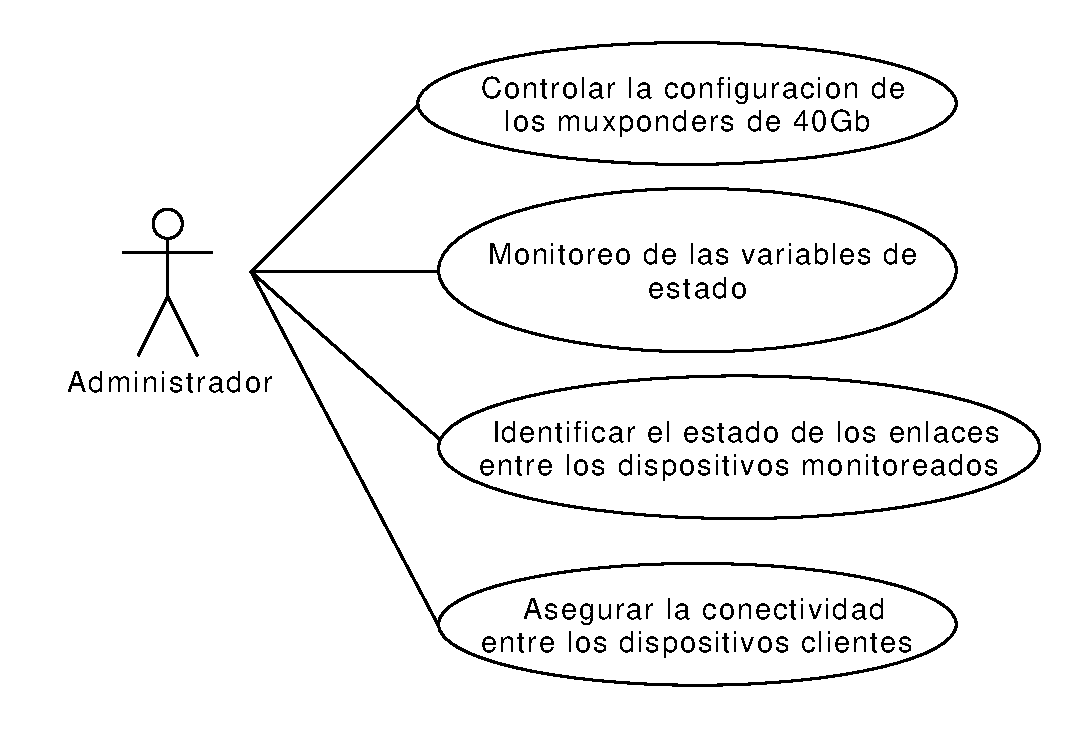
\includegraphics[scale=0.55]{Figures/caso_uso_admin.pdf}
    \caption{Caso de uso desde la perspectiva del administrador.}
    \label{fig:caso_uso_admin}
  \end{figure}

  En base a este diagrama, se pueden definir los requerimientos funcionales a nivel de sistema. La figura \ref{fig:req_sys} muestra una lista de los mismos. 
  
  Como requerimiento no funcional, se puede identificar la adición de nodos virtuales, los cuales no afectan a la funcionalidad del sistema pero brindan más flexibilidad y permiten conformar una topología más compleja.

  \begin{figure}[H]
    \centering
    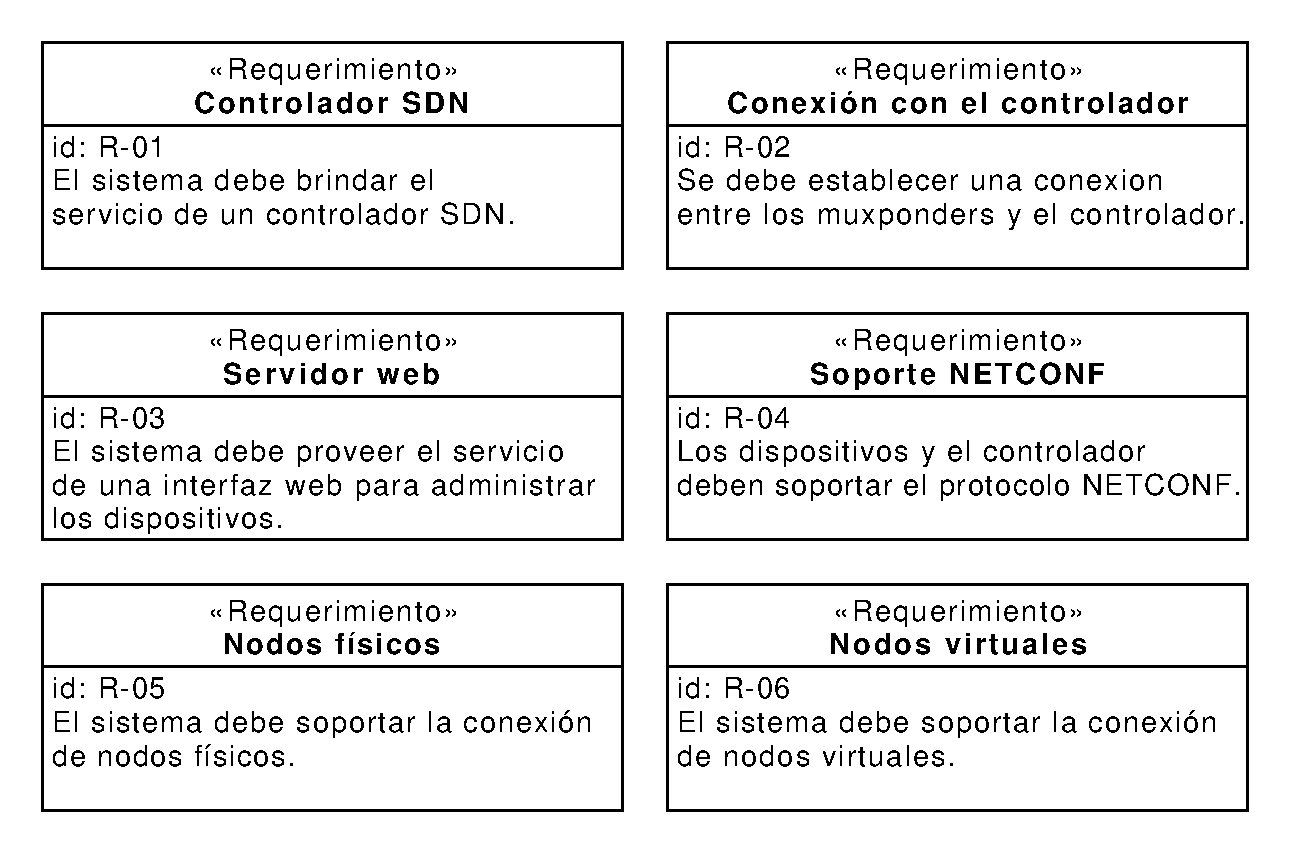
\includegraphics[scale=0.65]{Figures/req_sys.pdf}
    \caption{Requerimientos del sistema.}
    \label{fig:req_sys}
  \end{figure}


  Además, a partir del diagrama de caso de uso de la figura \ref{fig:caso_uso_admin}, se pueden identificar tres diagramas de actividades relacionadas. La figura \ref{fig:actividad_config}, muestra los flujos de actividad típicos que tendrá el sistema. 
  
  Para la actividad relacionada al monitoreo, la aplicación \textit{WEB} realiza consultas periódicas al controlador con el fin de obtener información sobre los dispositivos. Así, se envía un mensaje HTTP con la operación GET desde la aplicación, el controlador procesa la petición y responde dicha consulta.

Por otra parte, para el flujo de actividad relacionado a las notificiaciones, es el dispositivo quien emite inicialmente el mensaje mediante una notificación \textit{NETCONF}. El controlador, se procesa la notificación y se la registra como alarma.

Por último, se tiene el diagrama de actividad relacionado a la configuración del equipo. El evento inicial para este caso, es la adición de una configuración desde la aplicación \textit{WEB}. Esta configuración, una vez procesada, se traduce en una solicitud POST HTTP que se envían hacia la \textit{Northbound} interface del controlador. Una vez recibida la solicitud, se realiza su procesamiento y se envía el mensaje de configuración \textit{NETCONF} a los dispositivos involucrados a través de la \textit{Southbound} interface.


  


  \begin{figure}[!h]
    \centering
    \begin{subfigure}[b]{0.43\textwidth}
        \centering
        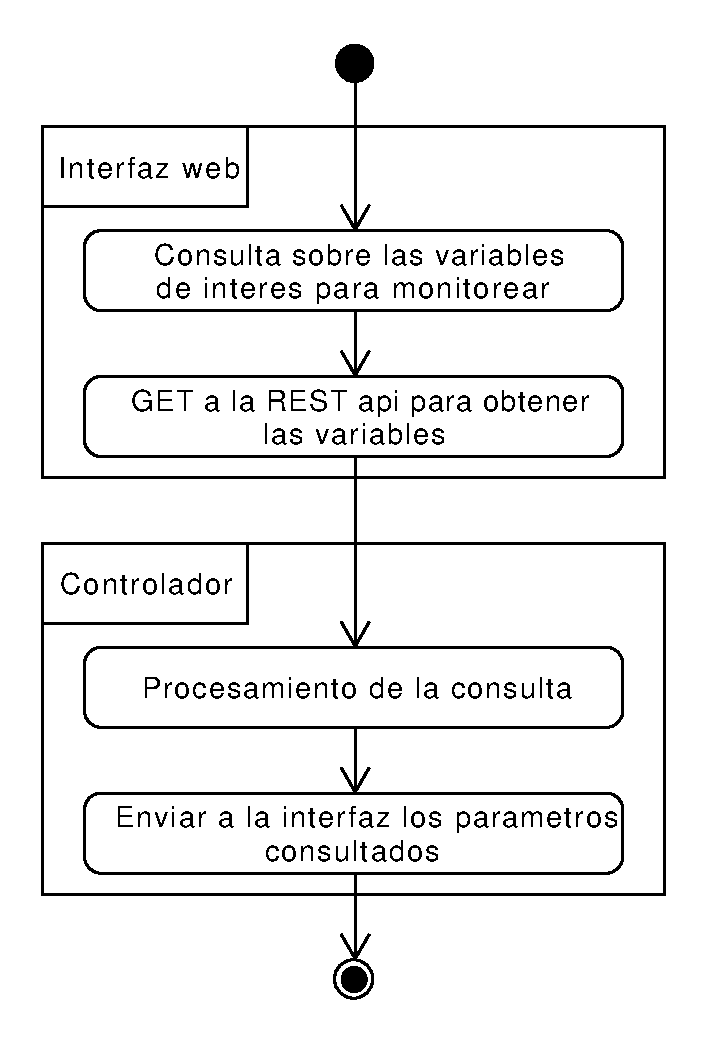
\includegraphics[width=\textwidth]{Figures/actividad_monitoreo.pdf}
        \caption{Actividad de monitoreo.}
    \end{subfigure}
    \quad
    \begin{subfigure}[b]{0.43\textwidth}  
        \centering 
        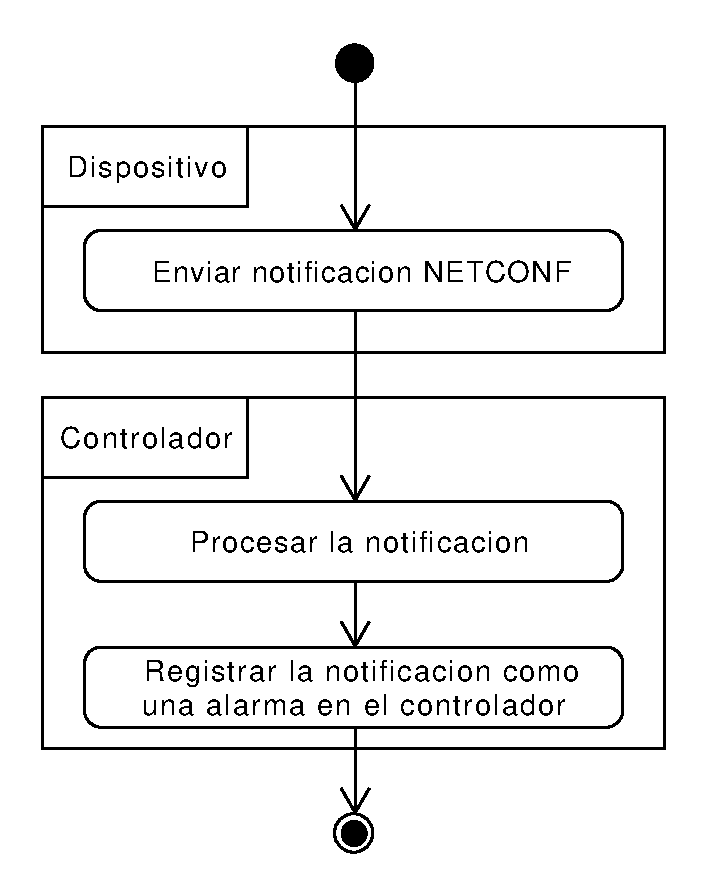
\includegraphics[width=\textwidth]{Figures/actividad_notif.pdf}
        \caption{Actividad de notificación.}
    \end{subfigure}
    \vskip\baselineskip
    \begin{subfigure}[b]{0.43\textwidth}   
        \centering 
        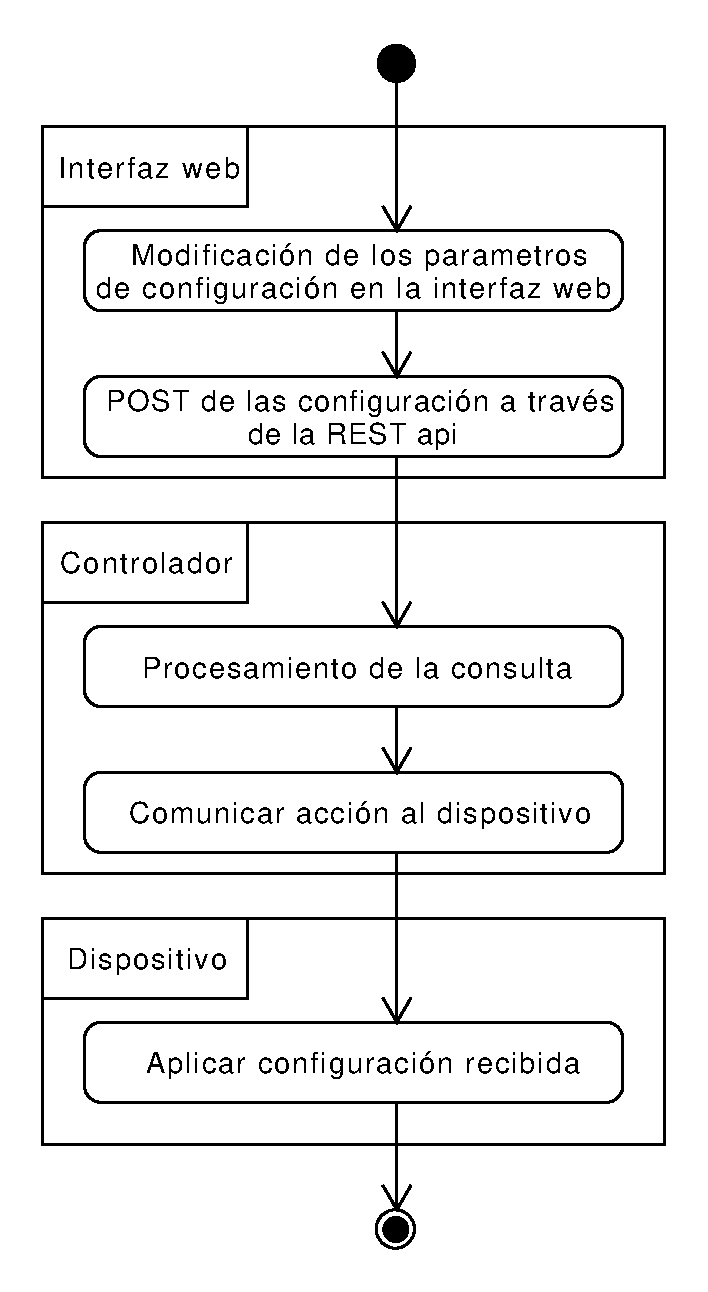
\includegraphics[width=\textwidth]{Figures/actividad_config_web.pdf}
        \caption{Actividad de configuración.}
    \end{subfigure}
    \caption{Diagramas de actividad del sistema.}
    \label{fig:actividad_config}
\end{figure}

\begin{comment}
  \begin{figure}[H]
    \centering
    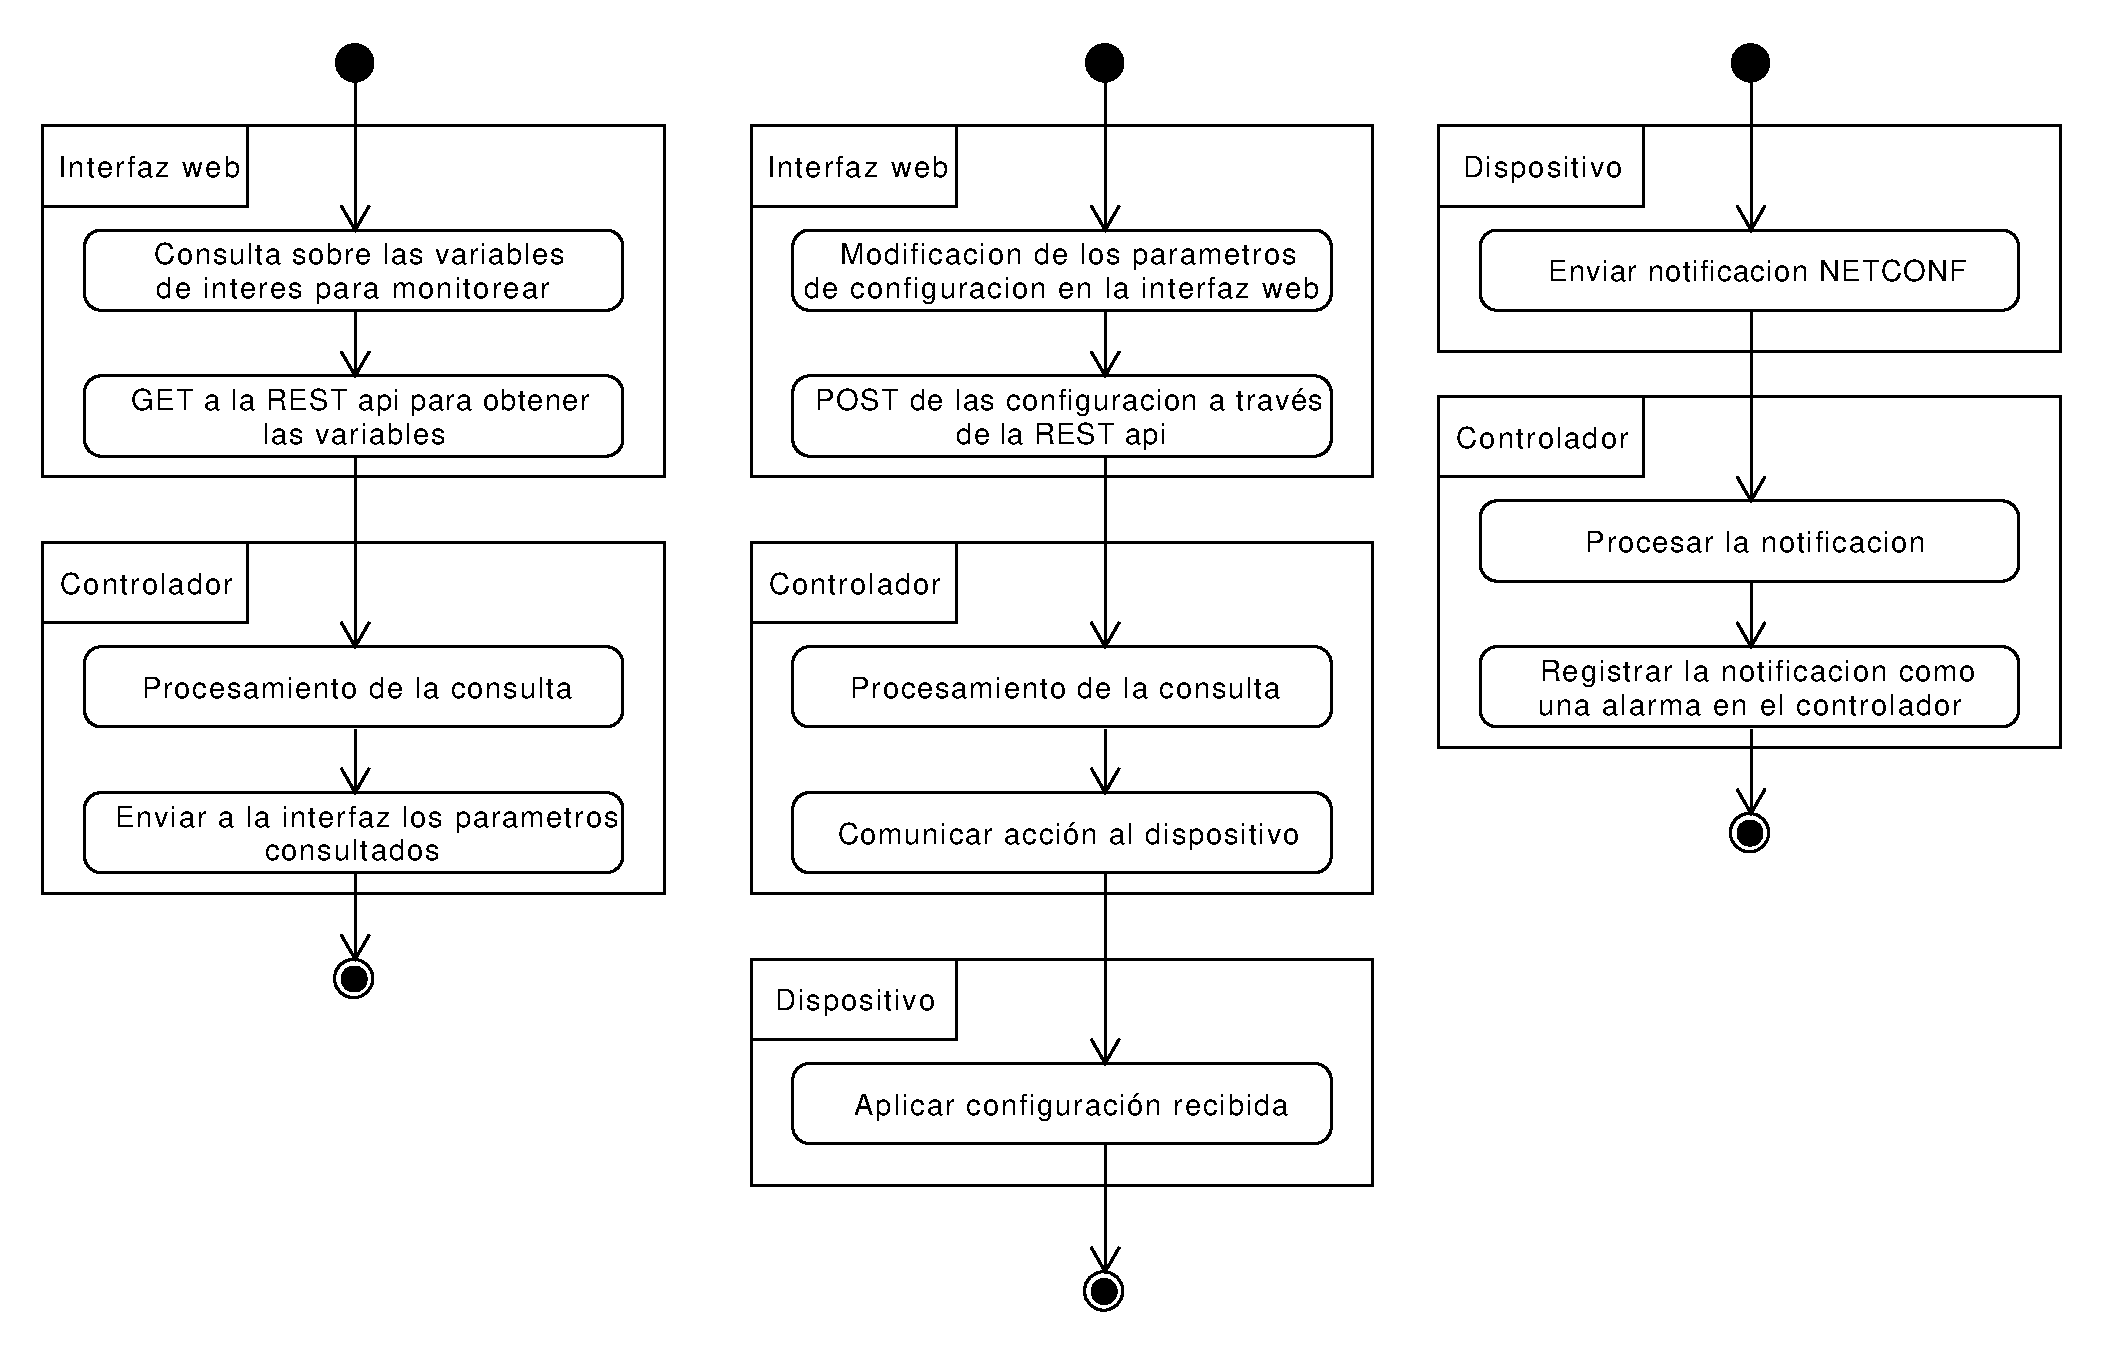
\includegraphics[scale=0.40]{Figures/actividad_config.pdf}
    \caption{Topología implementada en el proyecto.}
    \label{fig:actividad_config}
  \end{figure}
\end{comment}

\newpage
  %----------------------------------------------------------------------------------------
%	SECTION 2
%----------------------------------------------------------------------------------------

  \section{Integración del protocolo \textit{NETCONF} al \textit{muxponder}}
  La sección anterior deja claro que uno de los requerimientos de sistema será que tanto el controlador \textit{ONOS} como los dispositivos a monitorear, soporten \textit{NETCONF} como protocolo de gestión de la configuración. 
  
  Como se vio en el capítulo anterior, el controlador soporta dicho protocolo, por lo que para cumplir con este requerimiento de sistema, únicamente será necesario adaptar \textit{NETCONF} al dispositivo. 
  
  %-----------------------------------
%	SUBSECTION 1
%-----------------------------------

  \subsection{Requerimientos}

  Los requerimientos que deberá cumplir la integración del protocolo son los que se observan en la figura \ref{fig:req_netconf}.

  \begin{figure}[H]
    \centering
    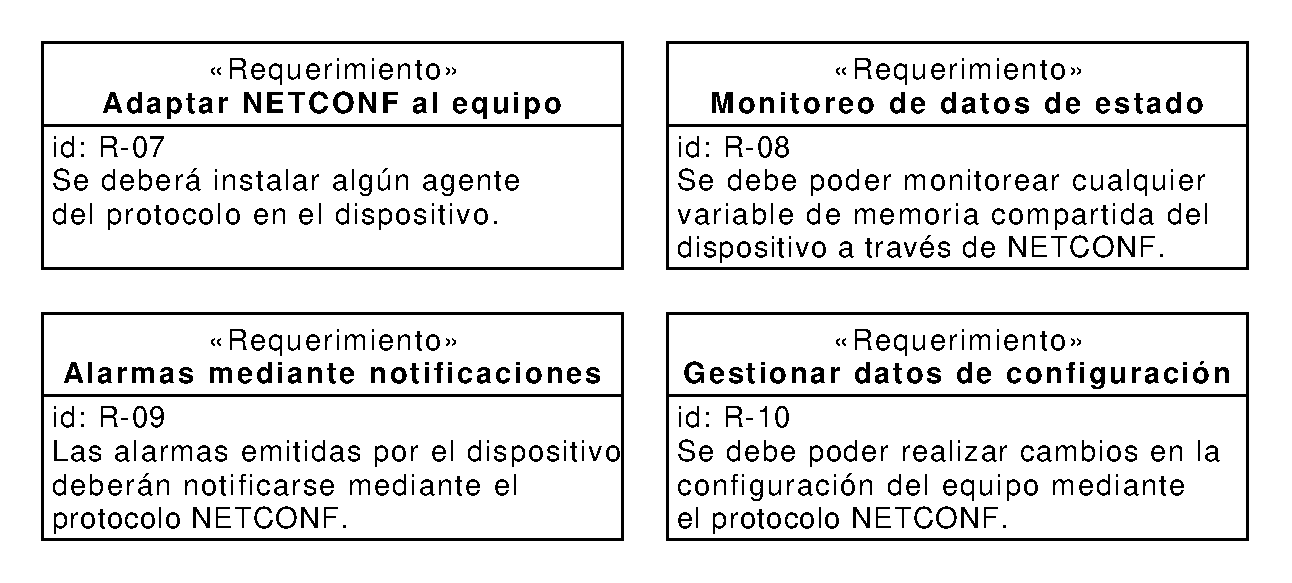
\includegraphics[scale=0.65]{Figures/req_netconf.pdf}
    \caption{Requerimientos para la integración del protocolo \textit{NETCONF}.}
    \label{fig:req_netconf}
  \end{figure}

%-----------------------------------
%	SUBSECTION 2
%-----------------------------------

  \subsection{Compilación e instalación del agente}
Siendo YUMA123 el agente que se eligió para integrar el protocolo en el equipo, en esta sección se detalla el procedimiento que se llevó a cabo para la compilación e instalación del agente en el \textit{muxponder}, con el fin de poder cumplir el requerimiento R-07.
\\

  En primer lugar, toda la tarea de compilación se realizó en una computadora de propósito general, debido a los recursos limitados con los que cuenta el dispositivo. Para facilitar la compilación e instalación, se realizaron tres scripts los cuales se describen a continuación:

  \begin{itemize}
	\item \textbf{\texttt{Dockerfile}}: el objetivo de este script, es el de realizar la compilación del proyecto YUMA123, dejando todas las librerías y los binarios en una carpeta que luego deberá copiarse en el dispositivo. Dockerfile \parencite{dockerfile}, es un archivo de texto que contiene los pasos e instrucciones que la herramienta Docker deberá seguir para construir una imagen. En el mismo, se indica una imagen de referencia (ubuntu:16.04) que servirá como base para la construcción. Luego, se descargan todas las librerías requeridas por el proyecto YUMA123 junto con los compiladores necesarios para realizar la compilación cruzada. A partir de aquí, se compila cada una de las librerías para la arquitectura objetivo (por ejemplo, NIOS II) y finalmente se compila también el proyecto YUMA123. Todos los binarios, librerías y cabeceras resultantes se encuentran en la carpeta “$/root/usrapp$” de la imagen Docker construida. Cabe destacar que se realizaron tres versiones del script, de esta forma compilar para las arquitecturas NIOS II, ARM y \texttt{x86\_64}.
    
    \item \textbf{\texttt{remote\_install\_yuma.sh}}: script bash que tiene la tarea de realizar la instalación del protocolo, compilado previamente con Docker y Dockerfile. Para ello, requiere de tres parámetros: usuario del dispositivo remoto, dirección IP del dispositivo remoto y la arquitectura deseada. Con estos parámetros, el script realiza la instalación del agente mediante SSH y SCP \parencite{scpman}, copiando el contenido necesario de "$/root/usrapp$" que se generó con la construcción de la imagen Docker, al directorio "$/root/usrapp$" del dispositivo. Es importante mencionar que muchas de las librerías requeridas por YUMA123 son necesarias únicamente para la compilación y no para el funcionamiento del protocolo, por lo que este script omitirá dichas librerías con el fin de reducir el tamaño que ocupa el agente en memoria.
    
    \item \textbf{\texttt{remote\_uninstall\_yuma.sh}}: requiere dos parametros los cuales son el usuario del dispositivo remoto y la dirección ip del mismo. El objetivo de este script es facilitar la desinstalación de todas las librerías relacionadas a YUMA123 del dispositivo.

\end{itemize}


\subsection{Diseño del módulo \textit{YANG}}

Para poder cumplir con los requerimientos R-08, R-09 y R-10 que se muestra en la figura \ref{fig:req_netconf}, se diseñó un módulo \textit{YANG} que contiene cinco secciones bien definidas, las cuales se describen a continuación: 

\begin{itemize}
	\item \textbf{Cabecera del módulo y declaraciones}: aqui se declara la estructura inicial del módulo \textit{YANG}. Se define un nombre y un prefijo, se realiza una descripción del mismo y por último se realiza la definición de los datos utilizados por el módulo. Cabe destacar que se definieron tres tipos de datos: restricted-tipo-trafico, restricted-tipo-fec-linea y restricted-tipo-fec-cliente. En ellos, se especifica a través de la directiva ‘enum’ cuales seran los valores aceptados que pueden tomar dichos tipos de datos. Por ejemplo, dado que la configuración del tipo de tráfico para este dispositivo únicamente admite dos valores (otu2 y xge), es importante restringir el ingreso de algún otro valor ya que podría ocasionar errores en la configuración. Se puede observar un fragmento de esta sección en la figura \ref{lstlisting:cabecera}, donde se detalla la cabecera del módulo y sus declaraciones.  

  \newpage
    \begin{lstlisting}[language=SHELXL, caption=Cabecera del módulo \textit{YANG}., label=lstlisting:cabecera]
        module cli-mxp {
            namespace "http://fulgor.com/ns/cli-mxp";
            prefix "cli-mxp";
            description
              "CLI para configurar el muxponder de 40G";
            revision "2018-06-24" {
                description
                  "Version 0.1.0";
            }

            typedef restricted-tipo-trafico {
                type enumeration {
                    enum "otu2";
                    enum "xge";
                  }
            }
              ...
              ...
              ...

    \end{lstlisting}

    \item \textbf{Container \textit{YANG} de configuración}: en esta sección se declara un container llamado ‘mux-config’. Aquí se describen todos los parámetros que admiten una configuración (por ejemplo, el tipo de fec de línea), a través de las declaraciones ‘leaf’. Un fragmento de esta sección puede observarse en la figura \ref{lstlisting:config_container}, donde además se puede ver el uso de los tipos de datos definidos en la cabecera del módulo.
  
    \begin{lstlisting}[language=SHELXL, caption=Container de configuración., label=lstlisting:config_container]
    container mux-config {
        description "Parametros de la CLI";

        leaf tipo_trafico {
            description
              "[otu2|xge] especifica el tipo de tráfico.";
            type restricted-tipo-trafico;
        }
      
      ...
      ...
      ...
        
        list ports {
            key "port";
            leaf port {
                type int16{
                    range "0 .. 6";
                }
                mandatory true;
            }

            leaf neighbor {
                mandatory true;
                type string;
            }
            
            leaf port_neighbor {
                mandatory true;
                type string;
            }
        }
    }
    \end{lstlisting}

    \item \textbf{Container \textit{YANG} de estado}: de igual forma, se realizaron containers para los datos de estado, los cuales no admiten una escritura de valores y son necesarios para monitorear el dispositivo. La figura \ref{lstlisting:state_container} muestra una parte de esta sección del módulo, donde puede apreciarse la directiva ’config false’, la cual indica que el container no admitirá datos de configuración.  

    \begin{lstlisting}[language=SHELXL, caption=Container de estado., label=lstlisting:state_container]
    container mux-state {
        description "Representa a datos de estado del dispositivo.";
        
        config false;

        leaf fpga_temperature_state {
            description "Temperatura de la FPGA";
            type decimal64 {
                fraction-digits 2;
            }
        }
   
        leaf device_boardId {
            description "Identificador unico del dispositivo";
            type string;
        }
        ...
        ...
        ...
    \end{lstlisting}


    \item \textbf{Definición de \textit{RPC}}: como se estudió en capítulos anteriores, \textit{NETCONF} permite definir \textit{RPC} propias de un módulo con el fin de extender la funcionalidad de los dispositivos. Se define así una \textit{RPC} cuya utilidad será la de poder indicar al agente cuándo debe aplicar la configuración que contiene el container 'mux-config' en el dispositivo. En la figura \ref{lstlisting:RPC}, se muestra dicha sección del módulo. En ella, se puede notar que la \textit{RPC} admite una respuesta de la operación solicitada, la cual está contenida en el leaf 'respuesta-mux-apply-config' y es de tipo String. En este mensaje se indica el resultado de la operación.

    

    \begin{lstlisting}[language=SHELXL, caption=Declaración de \textit{RPC}., label=lstlisting:RPC]
    rpc mux-apply-config {        
        description "RPC que aplica los cambios de configuracion";
        output {
            leaf respuesta-mux-apply-config {
                type string;
            }
        }
    }
    \end{lstlisting}

    \item \textbf{Definición de notificación}: por último, el módulo tiene una sección donde se declara una notificación. Dicho mensaje será utilizado para indicar a las sesiones conectadas y suscritas, las diferentes alarmas que produzca el dispositivo. Estos mensajes se transportan mediante notificaciones del protocolo \textit{NETCONF}. El propósito de estos mensajes es el de, por ejemplo, reportar mediante una alarma si un enlace con un dispositivo vecino se cayó, si el dispositivo supera la temperatura umbral, etc. La figura \ref{lstlisting:notif} muestra la declaración de dicha notificación en el módulo, donde se puede ver que el mensaje estará contenido dentro de la \textit{leaf} ’INFO’, en la cual se especifica de forma obligatoria con la directiva ’mandatory’ cuál será el mensaje que se enviará como notificación.

    \begin{lstlisting}[language=SHELXL, caption=Declaración de notificación., label=lstlisting:notif]
    notification mux-notify {
        leaf INFO {
            type string;
            mandatory "true";
        }
    }
    \end{lstlisting}

\end{itemize}

\subsection{Diseño de la librería C para el agente \textit{NETCONF}}
Con el objetivo comprender el funcionamiento de la librería desarrollada, será importante mencionar dos binarios que incorporan los \textit{muxponders} de 40Gb: 'monitor' y 'muxponder'. 

Para permitir que otros procesos conozcan el estado del dispositivo, el equipo utiliza el método de comunicación entre procesos llamado memoria compartida. El mismo, consiste en una región de memoria donde se permite que otras aplicaciones puedan, por ejemplo, leer información. 

Así, la aplicación 'monitor' es utilizada por el equipo para actualizar en dicha zona de memoria los valores de las diferentes variables a monitorear. Además, el binario mencionado también tiene la tarea de mostrar por la \textit{CLI} la información de estas variables. 

La figura \ref{fig:monitor} muestra la sección relacionada a los módulos XFP que produce en pantalla dicho binario en ejecución.

\begin{figure}[H]
    \centering
    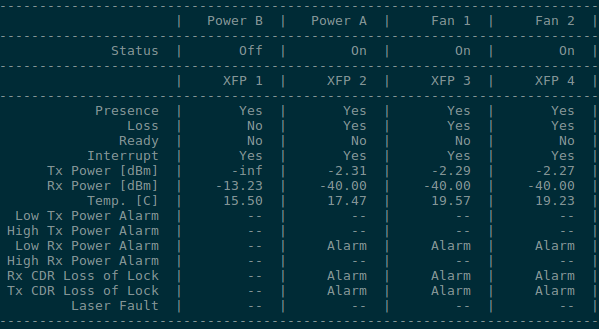
\includegraphics[scale=0.75]{Figures/monitorapp.png}
    \caption{Sección XFP de la aplicación ’monitor’.}
    \label{fig:monitor}
  \end{figure}

  Por otra parte, la aplicación 'muxponder' es utilizada por el administrador para poder configurar el dispositivo mediante ciertos parámetros que son especificados haciendo uso de la \textit{CLI} del equipo. Por ejemplo, con esta aplicación, el administrador podría cambiar la configuración de un equipo que tiene un tipo de tráfico $otu2$ por un tipo de tráfico $xge$ a través de la CLI, tal y como se muestra en la figura \ref{fig:mxpapp}.

  \begin{figure}[H]
    \centering
    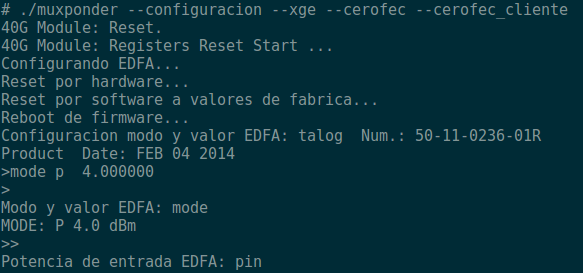
\includegraphics[scale=0.6]{Figures/muxponderapp.png}
    \caption{Configuración mediante la aplicación ’\textit{muxponder}’.}
    \label{fig:mxpapp}
  \end{figure}

  Teniendo en cuenta las aplicaciones mencionadas, se procede a explicar el diseño de la librería en el lenguaje C. Para ello, se utilizó la herramienta \textit{yangdump} del proyecto YUMA123, la cual genera un esqueleto de la aplicación a partir de un módulo \textit{YANG} dado. Se forman así dos archivos, uno con extensión '.h' (headers) y otro con extensión '.c' (código fuente). 
  

  En el primero, la herramienta declara todas las variables, funciones y los tipos de datos que va a utilizar la librería. 

  Por otra parte, el segundo archivo contiene la estructura de la aplicación en sí. En ella, se encuentran implementadas todas las funciones declaradas en el archivo con extensión '.h', las cuales llamará el agente en caso de que ingrese un mensaje referido al módulo \textit{YANG} en cuestión. Todo el desarrollo de la aplicación y la relación entre la instrumentación del dispositivo con el módulo \textit{YANG}, se encuentra en este archivo. 


  Con el fin de explicar cómo se desarrolló esta aplicación, se distinguen dos flujos de actividades bien definidos, uno para las operaciones que son sincrónicas con los mensajes que envía el cliente, y otro para aquellas que sean asíncronas a los mensajes del mismo. 

  Para el primer grupo, se tiene entonces las operaciones como obtención de un dato de estado o de configuración, modificación de un dato de configuración y ejecución de \textit{RPC}, mientras que el segundo grupo contempla el envío de notificaciones, las cuales son asíncronas a las operaciones del cliente.
  

  Se muestra el comportamiento de este primer grupo en el diagrama de actividad de la figura \ref{fig:actividad_modulo_sinc}. Cada vez que llega un mensaje \textit{NETCONF} al agente YUMA123, el mismo procesa y verifica a qué módulo \textit{YANG} hace referencia el mensaje y qué tipo de operación requiere el cliente. 

  Si la operación es una consulta por una variable de estado o de configuración, el agente realiza una llamada a una función relacionada a la variable consultada. En dicha función, lo que se hace es tomar el valor de memoria compartida del dispositivo, castear el mismo según indique el modulo \textit{YANG} (string, int, uint, etc) y por último, emitir una respuesta al cliente con el valor del dato consultado.

  Por otra parte, si la operación es la de editar una variable de configuración, el agente llama a una función de la librería C relacionada al módulo en cuestión, donde se actualiza el valor de dicha variable. Además, el agente emite un mensaje con el resultado de la operación. 

  Por último, si la operación trata de una \textit{RPC} definida en el módulo \textit{YANG}, el agente llama a la función relacionada a la \textit{RPC}, la cual contiene las instrucciones para efectuar la tarea solicitada. En este caso, se tiene una \textit{RPC} que indica cuándo se deberá aplicar la configuración en el dispositivo. Así, al momento de llamar a esta \textit{RPC}, el agente copia los valores de los datos de configuración necesarios (tipo de tráfico, tipo fec de cliente, tipo fec línea, etc) y los aplica haciendo uso del binario 'muxponder' explicado anteriormente.

  \begin{figure}[H]
    \centering
    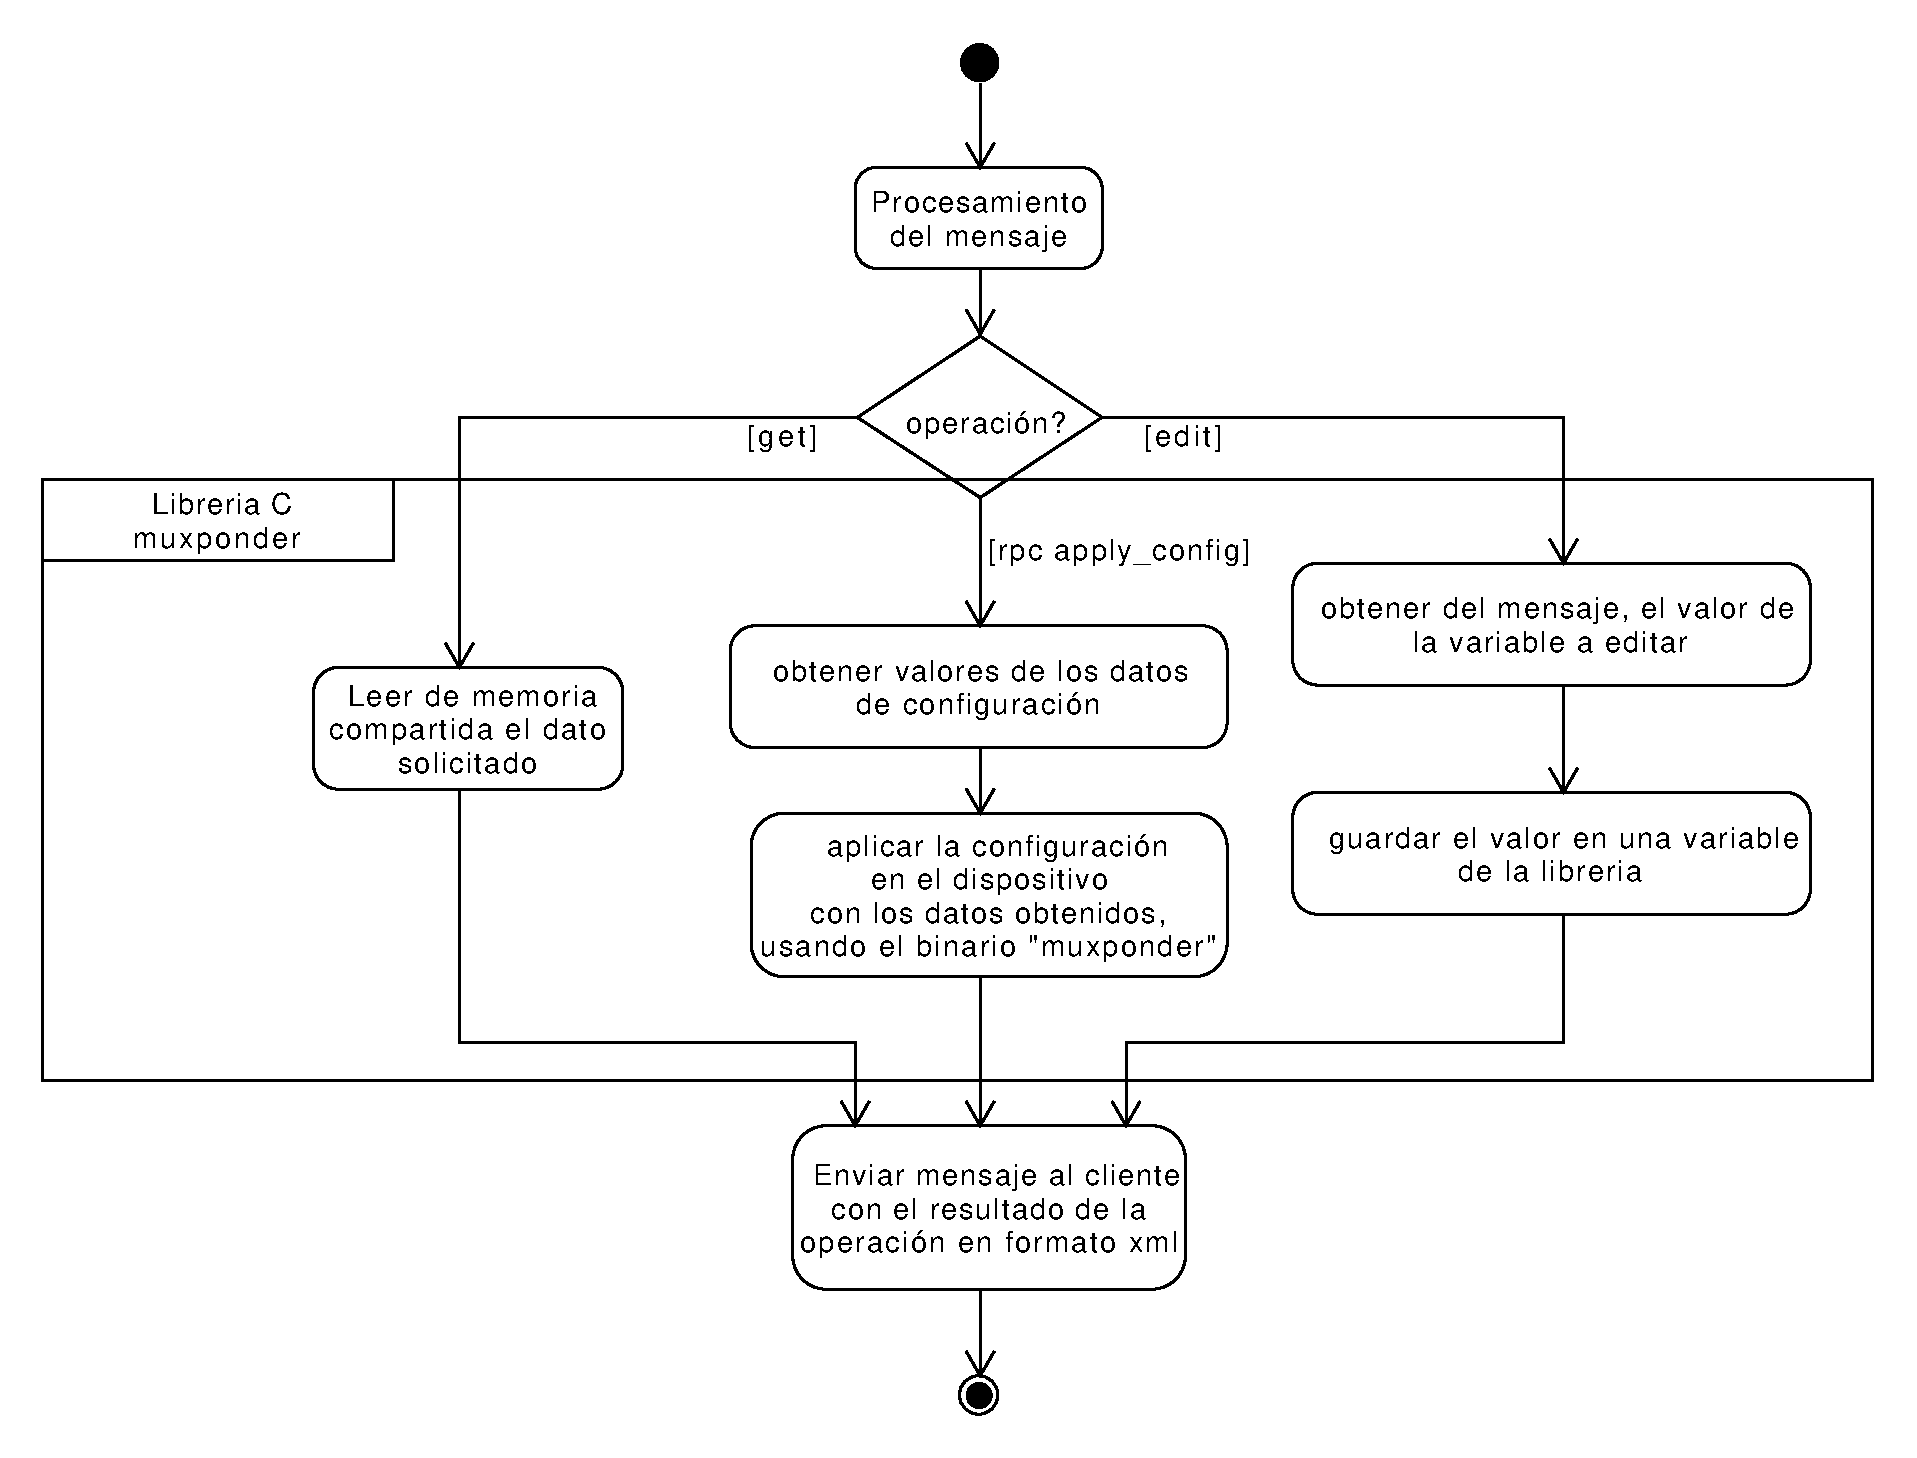
\includegraphics[scale=0.45]{Figures/actividad_modulo_sinc.pdf}
    \caption{Diagrama de actividad de las operaciones sincronas con el cliente.}
    \label{fig:actividad_modulo_sinc}
  \end{figure}

  Por otra parte, el grupo relacionado a las operaciones asíncronas con los mensajes del cliente, no es otra cosa que la operación de envío de notificaciones mediante el protocolo \textit{NETCONF}. Para ello, la librería desarrollada en C crea un hilo que examina periódicamente cada tres segundos la memoria compartida del dispositivo. 
  
  La razón por la cual se examina cada tres segundos, está relacionada con la aplicación 'monitor', la cual actualiza los valores de memoria compartida con esa frecuencia.

  Al examinar los valores de las alarmas, las compara con la información antigua que se tenía almacenada sobre las mismas. Si la información es igual, no se envían notificaciones a las sesiones. En cambio, si la información actual es diferente a la información anterior, será necesario notificar a las sesiones suscritas este nuevo estado de las alarmas. Así, tanto el nombre de la alarma como su nuevo estado, son enviados a través de la notificación definida en la figura \ref{lstlisting:notif}, haciendo uso de la \textit{leaf} INFO.
  
  Un diagrama de actividad de estas operaciones se puede observar en la figura \ref{fig:actividad_modulo_notif}.

  \begin{figure}[H]
    \centering
    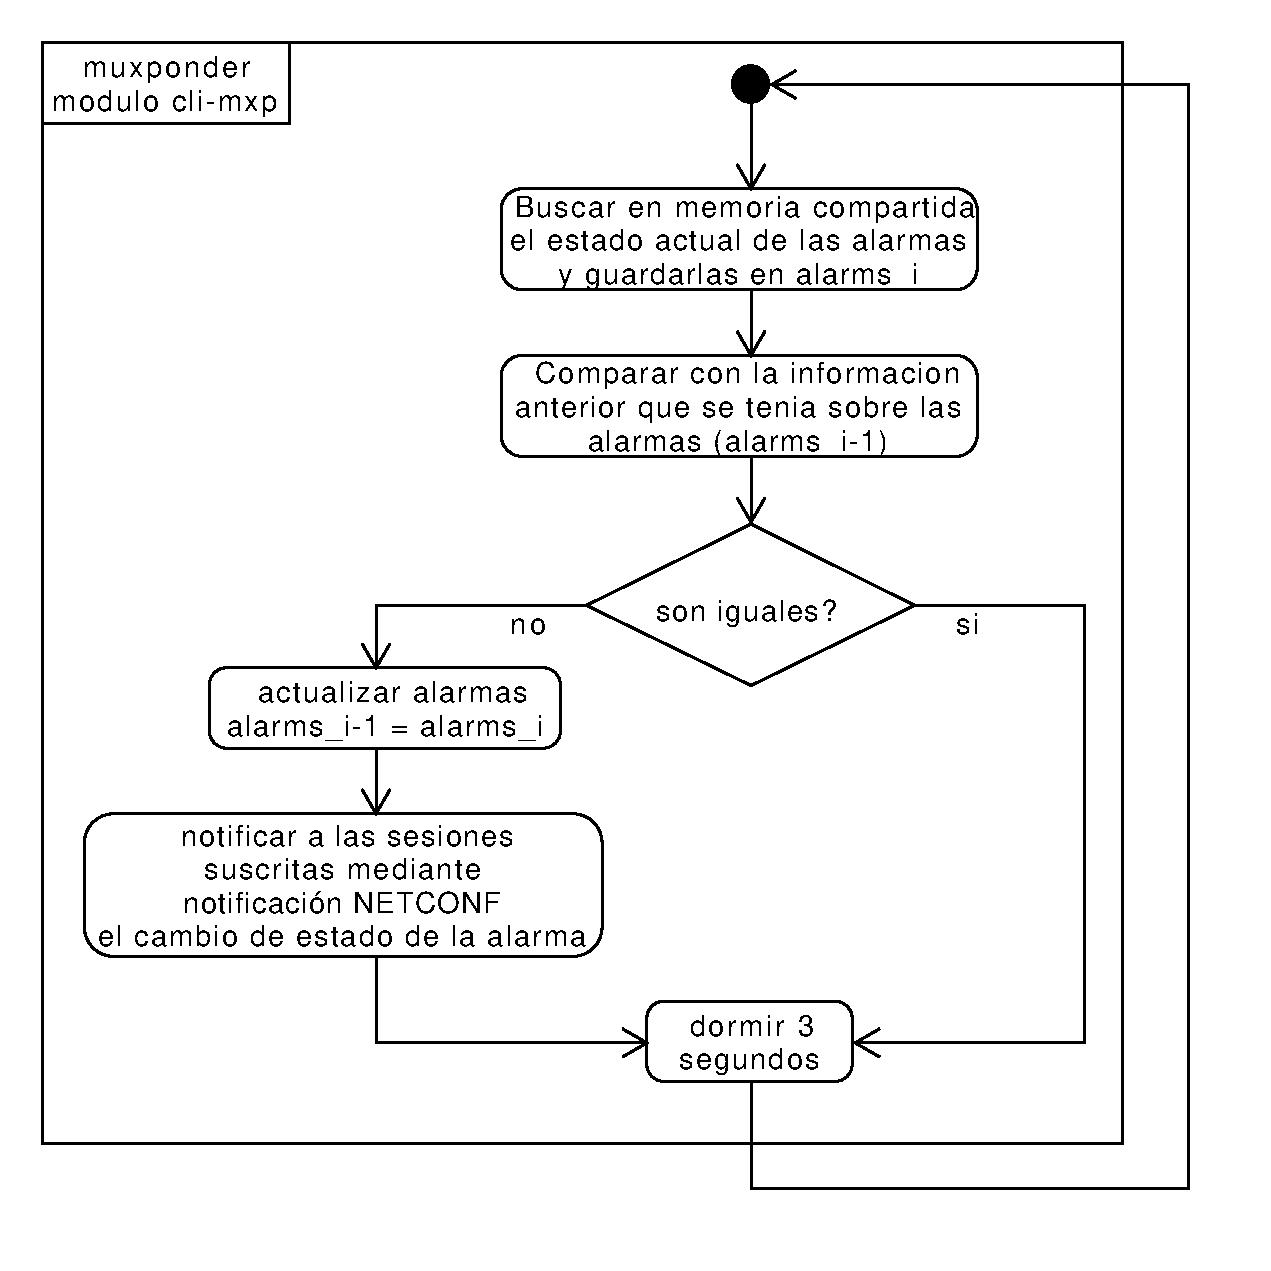
\includegraphics[scale=0.50]{Figures/actividad_modulo_notif.pdf}
    \caption{Diagrama de actividad de las notificaciones.}
    \label{fig:actividad_modulo_notif}
  \end{figure}


  \section{Diseño del \textit{driver}}
  Como se vio en capítulos anteriores, \textit{ONOS} se comunica con los dispositivos a través de tres componentes de la interfaz \textit{Southbound}: \textit{Providers}, \textit{Protocols} y \textit{Drivers}.
  
  Así, para poder indicar al controlador cuáles serán las operaciones y los comportamientos específicos del \textit{muxponder} de 40Gb, será necesario desarrollar un \textit{driver} (Java) en la interfaz \textit{Southbound} del controlador. 

  \subsection{Requerimientos}
  A fin de cubrir las necesidades del administrador, visto en el caso de uso de la figura \ref{fig:caso_uso_admin}, el \textit{driver} desarrollado deberá cumplir con los requerimientos funcionales de la figura \ref{fig:req_driver}.
  
  \begin{figure}[H]
    \centering
    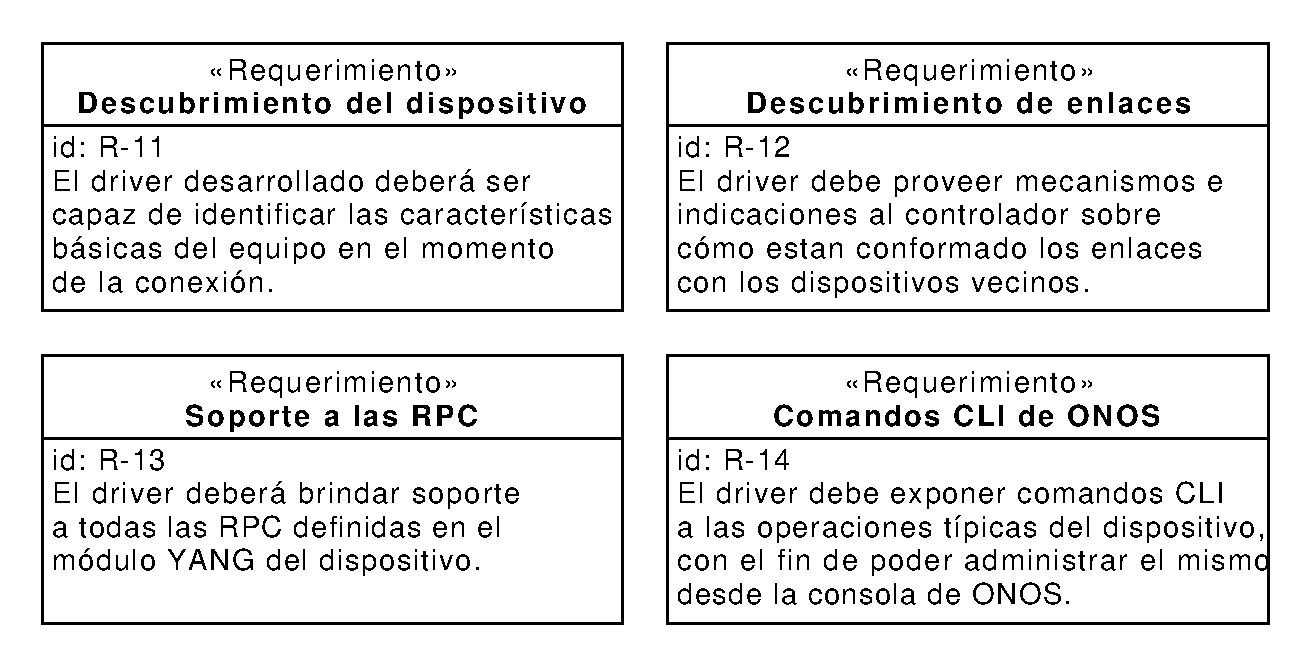
\includegraphics[scale=0.65]{Figures/req_driver.pdf}
    \caption{Requerimientos para el \textit{driver} de la interfaz \textit{Southbound}.}
    \label{fig:req_driver}
  \end{figure}

  \subsection{Descubrimiento del dispositivo}
  El controlador \textit{ONOS} reconoce la presencia de un nuevo dispositivo a través de un mensaje en formato JSON, el cual contiene información como la dirección IP del equipo, el \textit{driver} que describe sus comportamientos, el protocolo que utiliza, entre otra información de utilidad. 
  
  Un ejemplo de este mensaje se muestra en la figura \ref{lstlisting:JSON}. Dicho mensaje, es enviado al controlador haciendo uso del comando de \textit{ONOS} 'onos-netcfg' \parencite{onosconfserv}.

  \begin{lstlisting}[language=SHELXL, caption=Mensaje JSON con información del dispositivo., label=lstlisting:JSON]
    {
        "devices": {
            "netconf:172.16.0.141:830": {
            "netconf": {
                "ip": "172.16.0.141",
                "port": 830,
                "username": "user",
                "password": "pass",
            },
            "basic": {
                "driver": "altura-netconf"
           }
        }
    }
    \end{lstlisting}


    Al momento de indicar al controlador \textit{ONOS} la presencia de un nuevo dispositivo, el mismo hace una llamada por única vez a la función DeviceDescriptionDiscovery, la cual se encuentra implementada en el \textit{driver} indicado por el archivo JSON. 

    Esta función, tiene la tarea de descubrir las características más generales del equipo, como ser la versión de \textit{software} y de \textit{hardware} del mismo, el número de puertos disponibles, el identificador único del dispositivo, etc.

    Con más detalle, la función inicia la sesión SSH del protocolo \textit{NETCONF}, espera a que termine el intercambio de capacidades entre cliente y servidor y por último envia un mensaje \textit{NETCONF} al servidor, solicitando con la operación 'GET' los siguientes datos de estado:  
    
    \begin{itemize}
        \item información del fabricante.
        \item versión de \textit{hardware}.
        \item versión de \textit{software}.
        \item identificador único del equipo.
        \item alarmas activas en el equipo.
    \end{itemize}


    La figura \ref{fig:actividad_driver_descr} muestra el flujo de actividad típico que tendría el controlador \textit{ONOS} al momento de agregarse un nuevo dispositivo administrado por el \textit{driver} desarrollado.
    
    \begin{figure}[H]
        \centering
        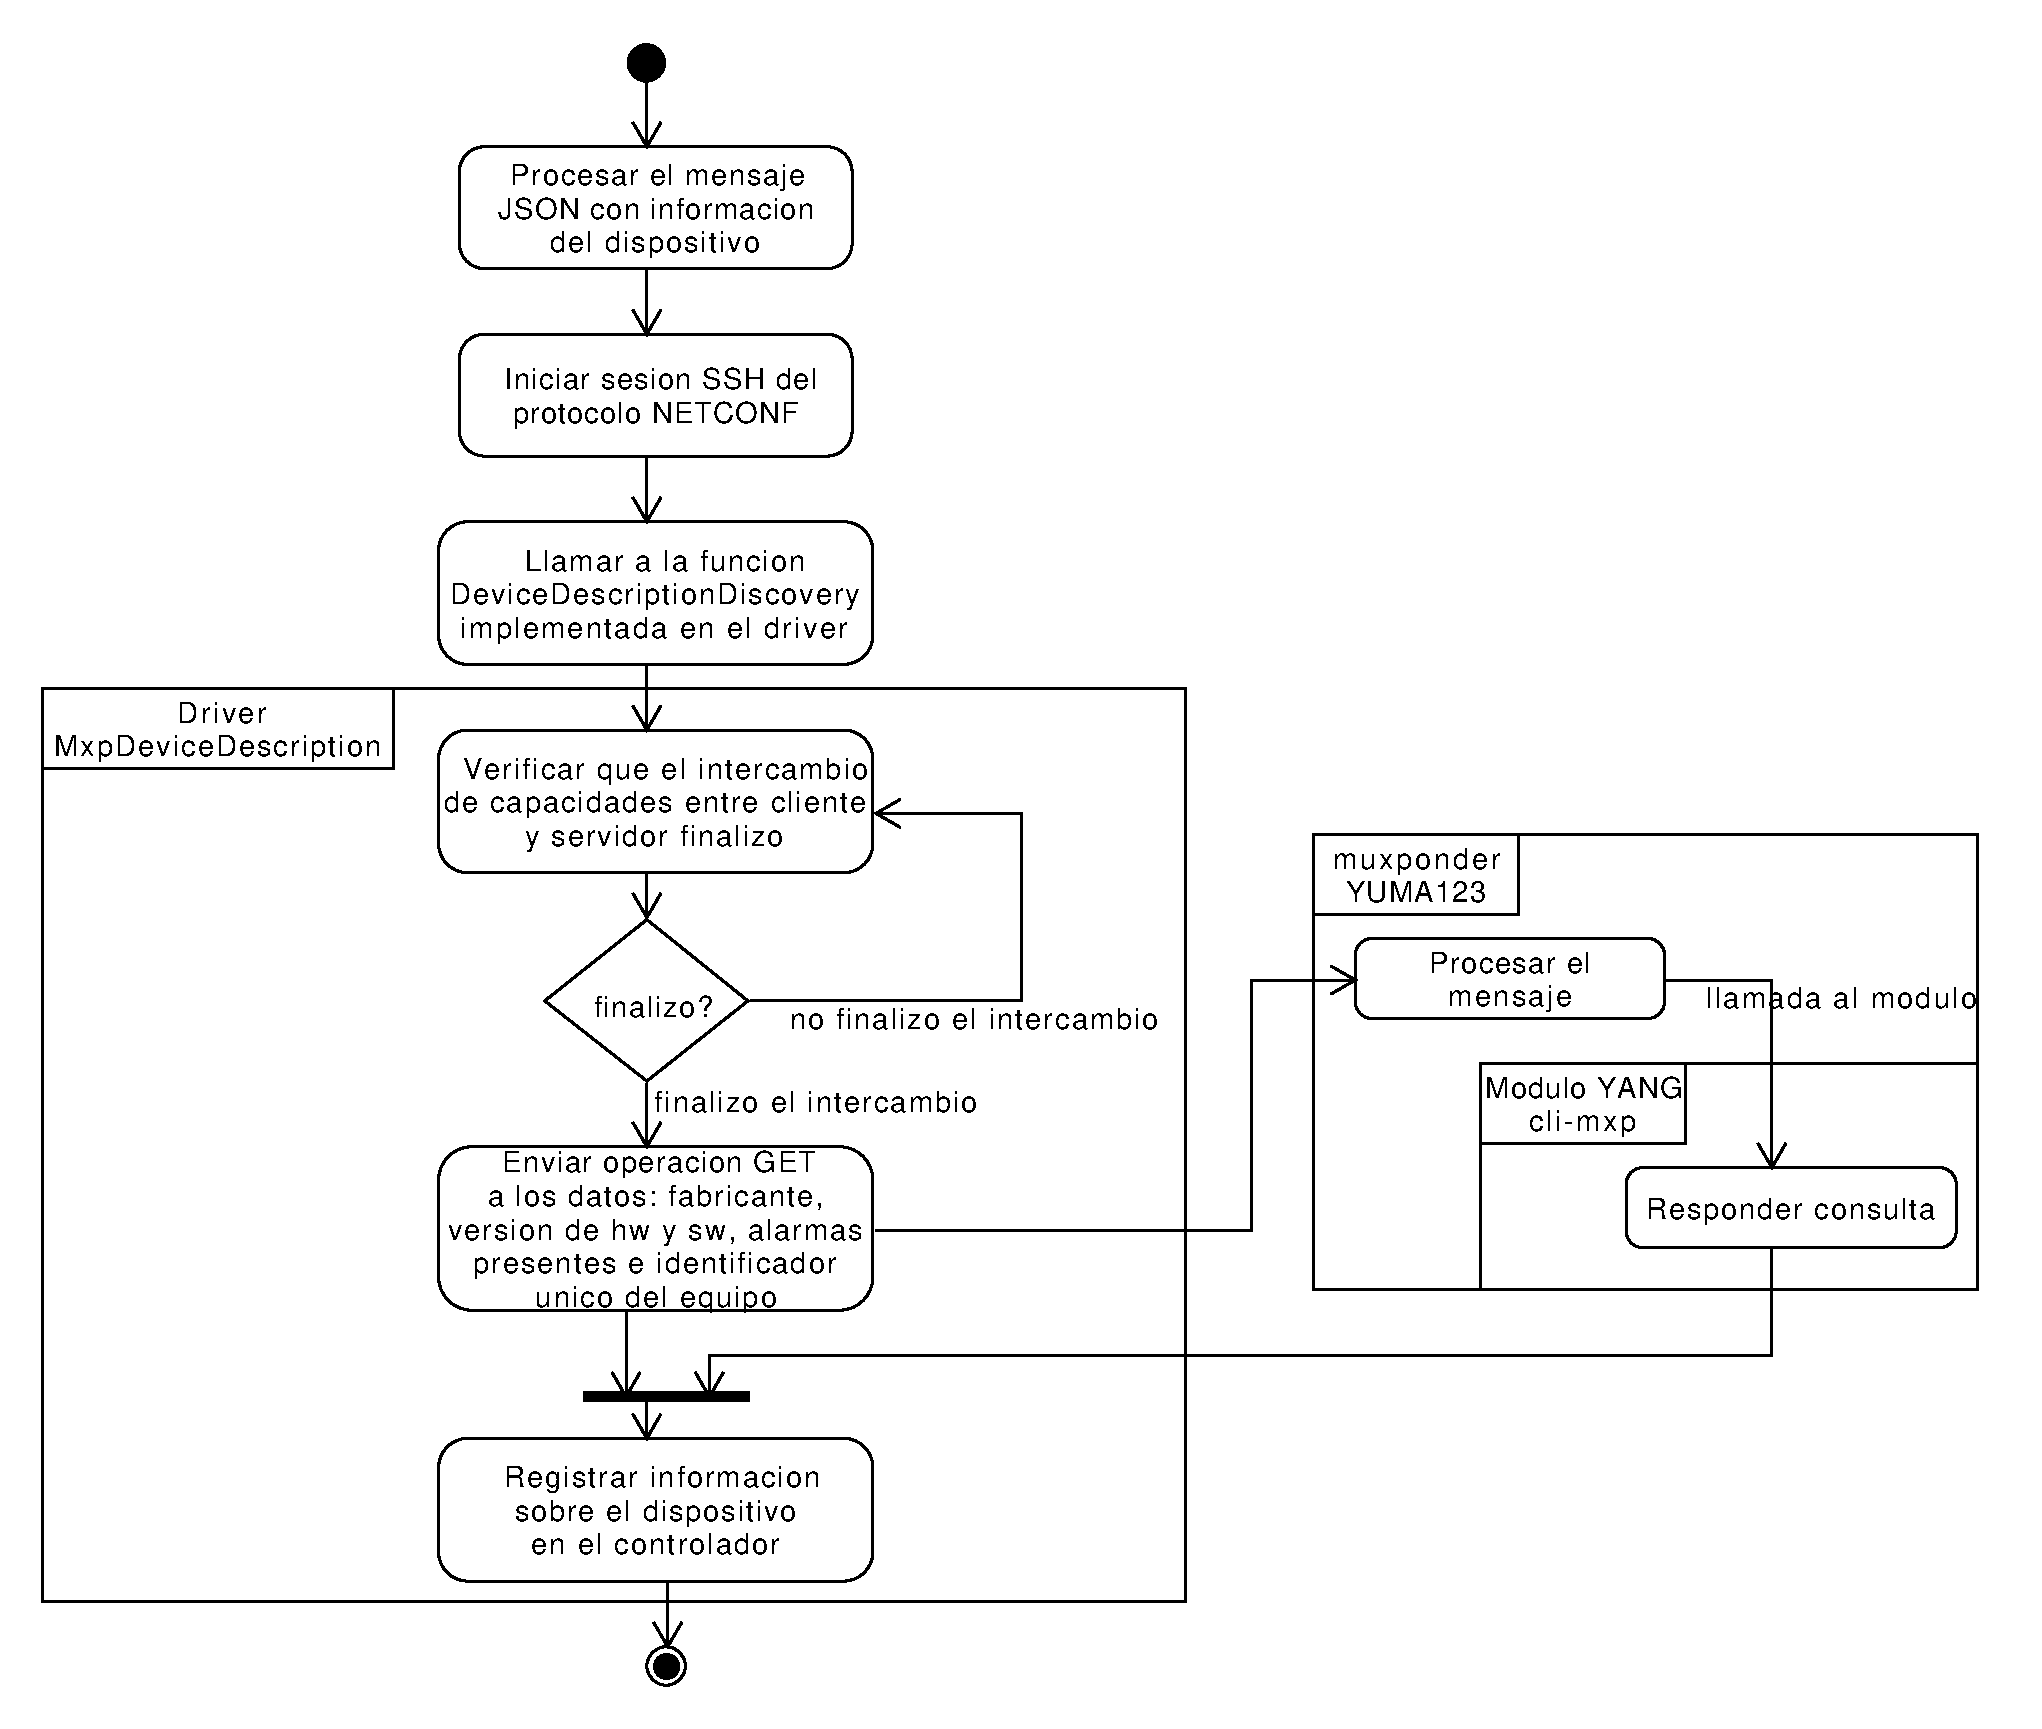
\includegraphics[scale=0.45]{Figures/actividad_driver_descr.pdf}
        \caption{Diagrama de actividad de la función DeviceDescriptionDiscovery.}
        \label{fig:actividad_driver_descr}
      \end{figure}

\subsection{Descubrimiento de Enlaces}

El \textit{driver} también debe proveer un mecanismo para indicar al controlador cómo se componen los enlaces entre los diferentes dispositivos administrados. Para ello, el controlador \textit{ONOS} brinda una interfaz llamada 'LinkDiscovery', la cual se deberá implementar en el \textit{driver}. 

Así, el controlador llama periódicamente a esta función (cada 30 segundos de forma predeterminada, pudiéndose cambiar este tiempo desde la CLI) para corroborar el estado de los enlaces. 

Con más detalle, lo que realiza esta función es enviar periódicamente a los dispositivos un mensaje \textit{NETCONF} con la operación GET-CONFIG, consultando por los datos “port”, “neighbor” y “port-neighbor” del container mux-config, estos datos pueden verse representados en el módulo \textit{YANG}, en la figura \ref{lstlisting:config_container}. A continuación, se explica de forma breve la función de cada uno de estos datos:

\begin{itemize}
	\item \textbf{port}: indica el puerto del dispositivo local al cual se conectará un vecino.
    
    \item \textbf{neighbor}: contiene el identificador único del dispositivo vecino.
    
    \item \textbf{port-neighbor}: indica el puerto del dispositivo vecino que se conectará en 'port' y con el que deberá formar el enlace.
\end{itemize}

Con esta información, el \textit{driver} informa al controlador que forme un enlace óptico entre ambos dispositivos. Si alguno de los dispositivos involucrados contiene alarmas registradas respecto al enlace de línea del muxponder, concretamente alarmas relativas al receptor, el enlace no se forma. El diagrama de actividad de la figura \ref{fig:actividad_link} muestra lo explicado anteriormente.

\begin{figure}[!h]
    \centering
    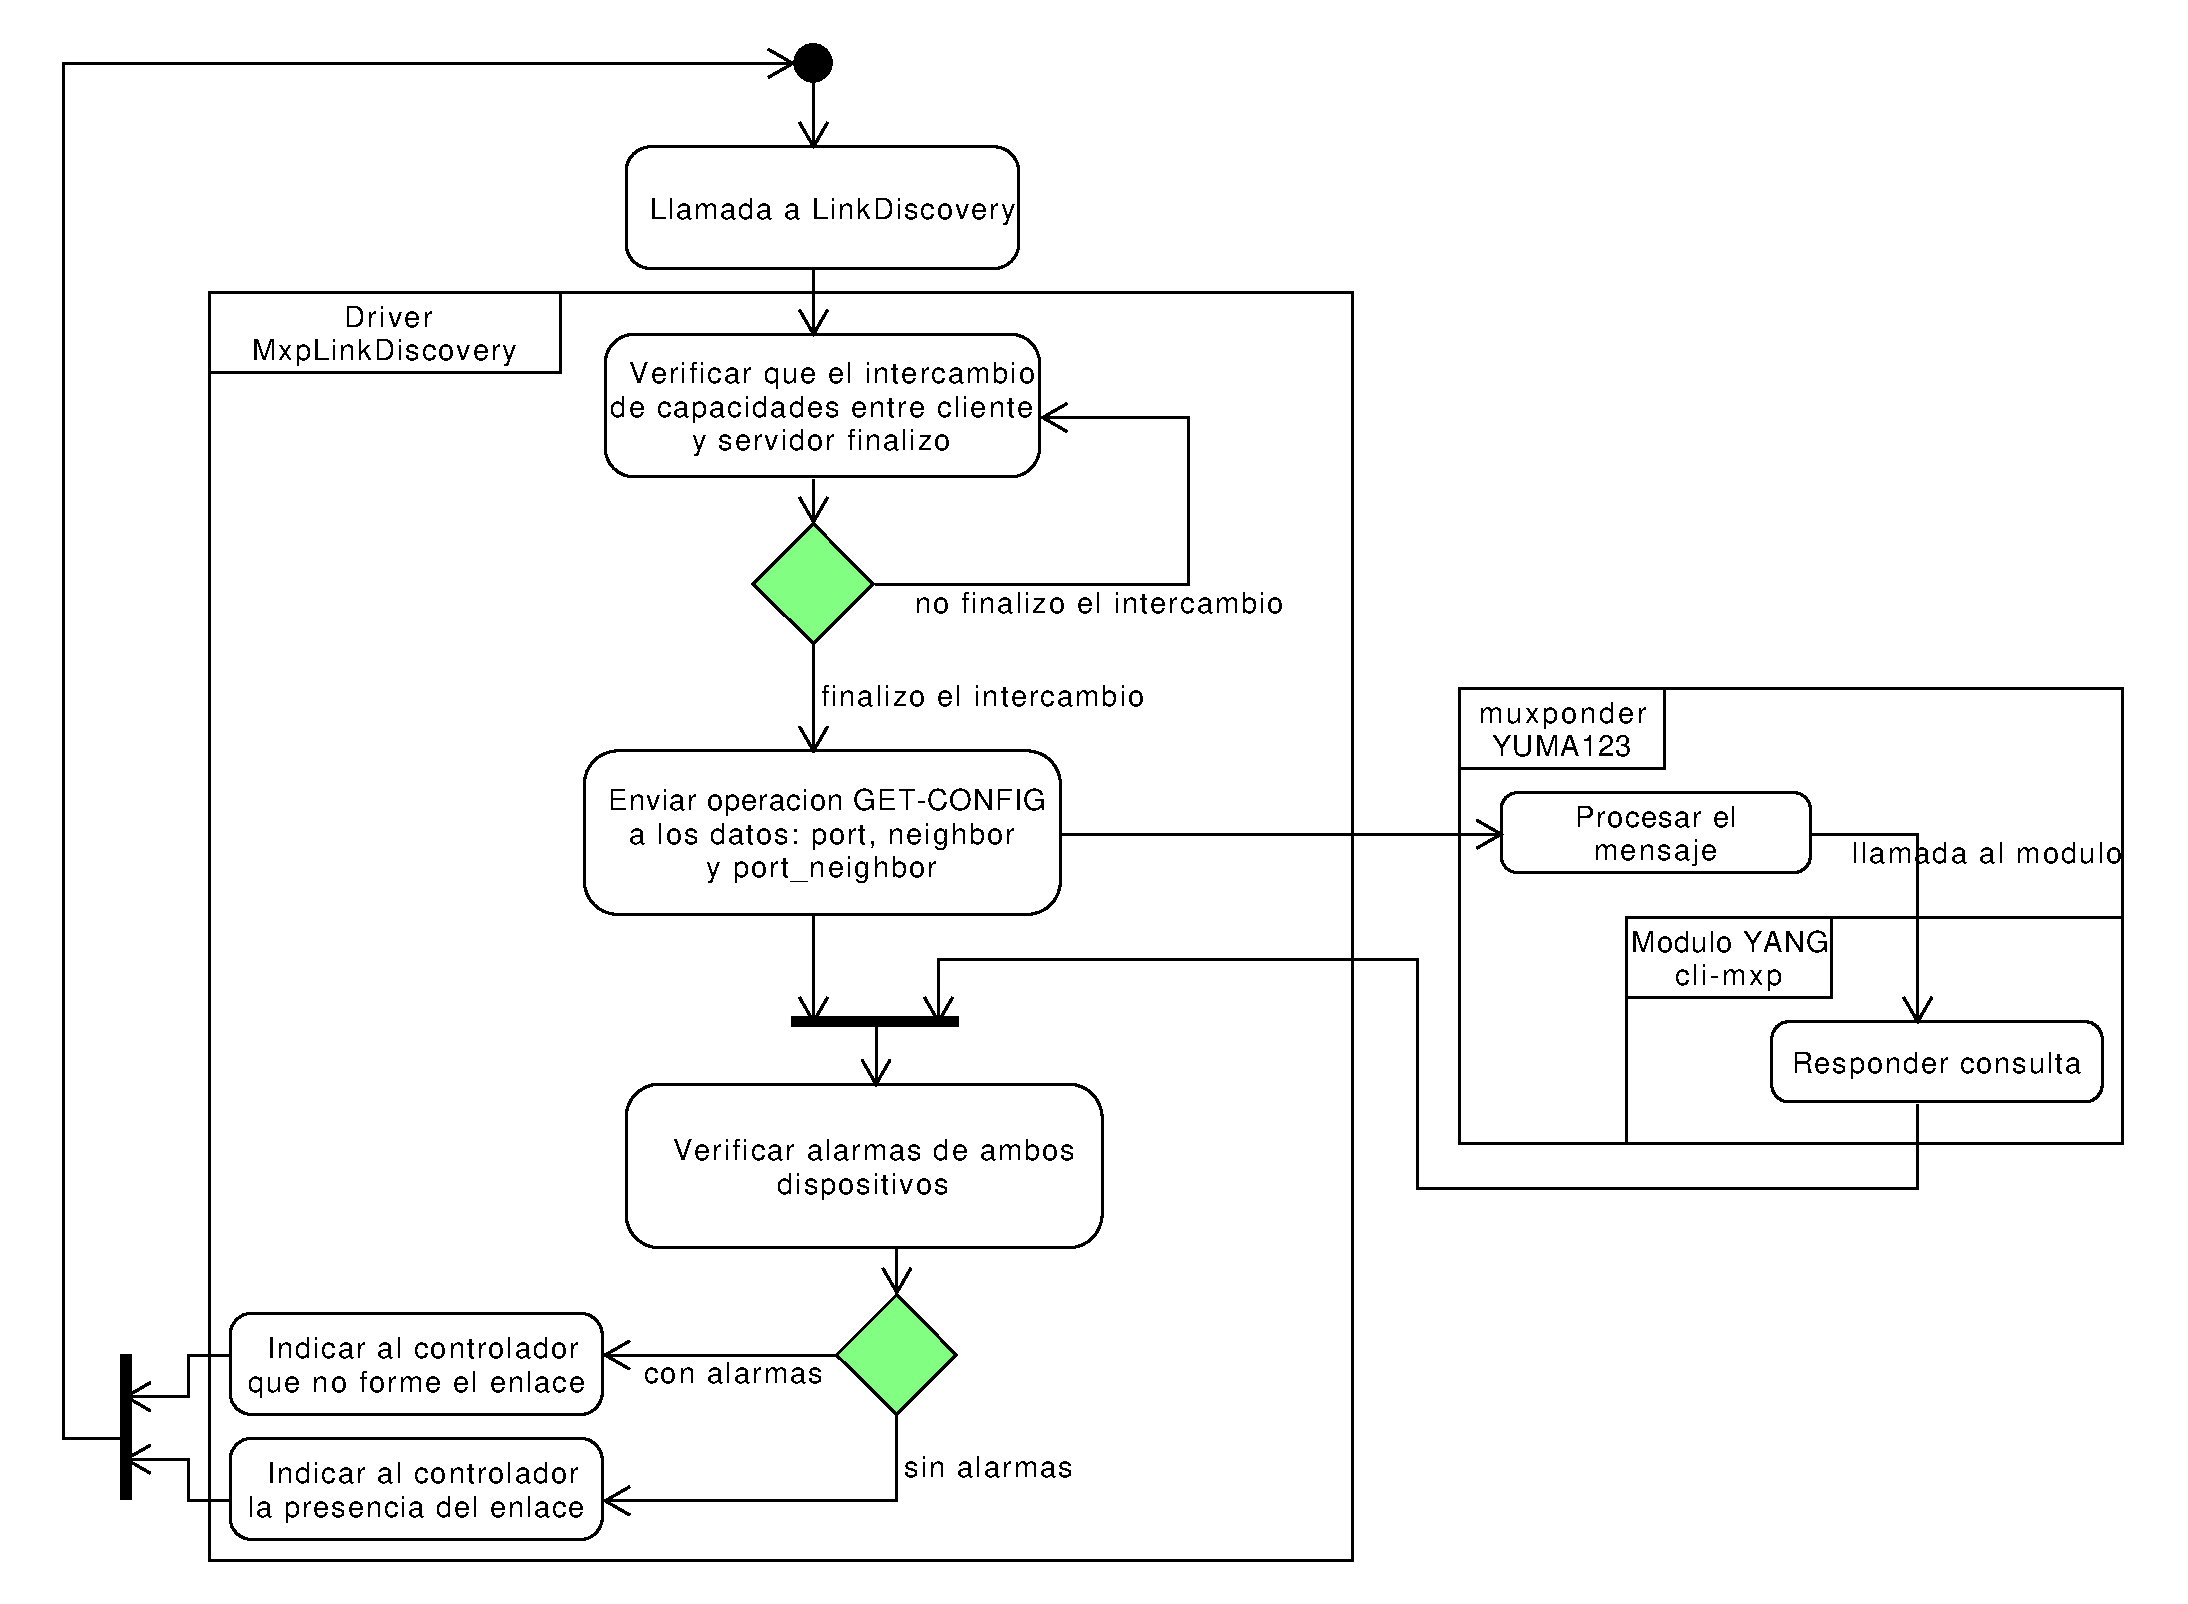
\includegraphics[scale=0.43]{Figures/actividad_link.pdf}
    \caption{Diagrama de actividad de la función LinkDiscovery.}
    \label{fig:actividad_link}
  \end{figure}

  Es importante mencionar que en esta instancia, no se consulta al dispositivo por sus alarmas con un mensaje \textit{NETCONF}, ya que las mismas son enviadas asíncronamente mediante notificaciones por el dispositivo, y registradas por el controlador como alarmas. Por lo tanto, para verificar el estado de las alarmas de un dispositivo, solo se consulta internamente en el core de \textit{ONOS}.

  \subsection{Operaciones definidas en el \textit{driver}}

  El \textit{driver} desarrollado brinda, además de las implementaciones de LinkDiscovery y DeviceDescriptionDiscovery explicadas anteriormente, la posibilidad de ejecutar cualquier operacion admitida por el modulo del dispositivo, entre ellas la \textit{RPC} que se describió en la figura \ref{lstlisting:RPC}. 
  
  Además, se especifican comandos \textit{CLI} para que el administrador pueda interactuar con los dispositivos a través del \textit{driver}, haciendo uso de la consola de \textit{ONOS}. 

  Se explica así el funcionamiento de la interfaz implementada para la operación \textit{RPC} “mux-apply-config”. 
  
  En el driver, esta función tiene una utilidad más además de indicar al dispositivo que tiene que aplicar la configuración. Dado que se puede indicar la presencia de dispositivos vecinos, es necesario corroborar que la configuración aplicada entre ellos sea la misma para garantizar la conectividad entre los clientes conectados a los \textit{muxponders}. Así, si se aplica una configuración en un \textit{muxponder}, el controlador deberá corroborar que los dispositivos vecinos conectados tengan la misma configuración aplicada, de lo contrario se deberá generar y registrar una alarma en el controlador.
  
  Teniendo en cuenta esto, el diagrama de la figura \ref{fig:actividad_driver_rpc_sin_vecinos} muestra el flujo de actividad que sigue el \textit{driver} cuando recibe una llamada a esta \textit{RPC} para el \textit{muxponder} A. Para este primer caso, el \textit{muxponder} A no tiene especificado ningún vecino, por lo que no se generará alguna alarma sobre configuración inconsistente, de hecho, se verifica que no tenga alarmas de este tipo y de tenerlas se eliminan.

  En primer lugar, cuando se llama a la función rpcApplyConfig, el \textit{driver} envía un mensaje al dispositivo con la operación \textit{RPC} que define el módulo \textit{YANG}. El agente YUMA123 recibe este mensaje, lo procesa y aplica la configuración en el equipo haciendo uso de los datos de configuración que tenga el datastore running. Por último, se envía un mensaje con la respuesta de esa operación. 

  Luego, el \textit{driver} consulta al mismo \textit{muxponder} si tiene algún vecino conectado, como en este caso no se tiene ningún vecino conectado, se eliminan las alarmas (si existe alguna) relacionadas al \textit{muxponder} A con configuración inconsistente entre los vecinos.

  \begin{figure}[H]
    \centering
    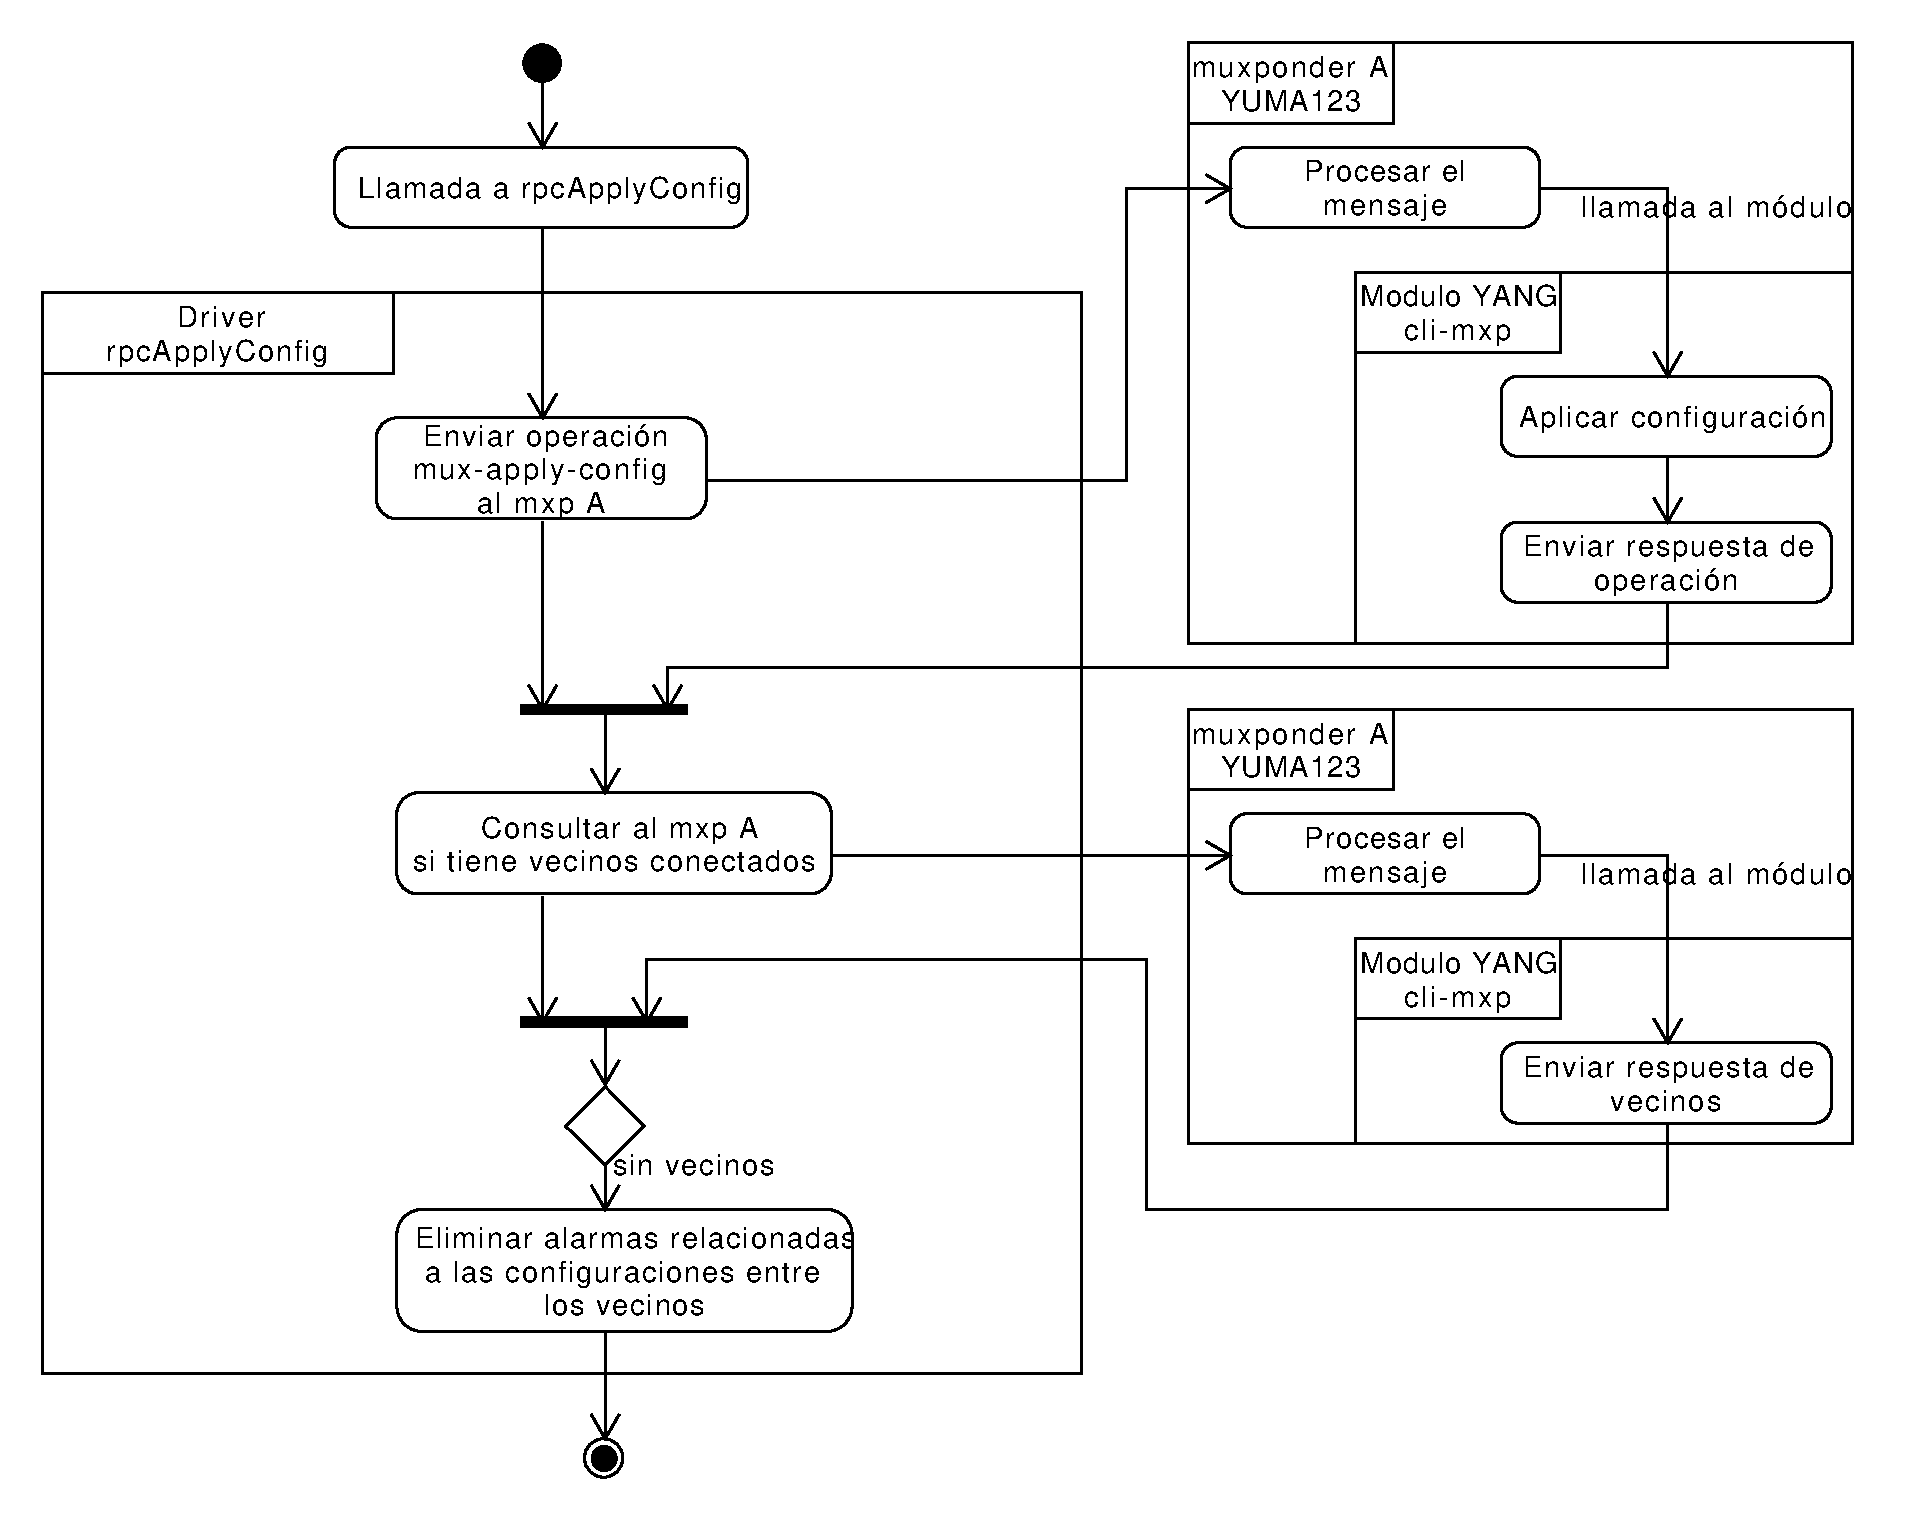
\includegraphics[scale=0.45]{Figures/actividad_driver_rpc_sin_vecinos.pdf}
    \caption{Diagrama de actividad para la \textit{RPC} mux-apply-config, sin vecinos.}
    \label{fig:actividad_driver_rpc_sin_vecinos}
  \end{figure}

  En caso de que el \textit{muxponder} A tenga vecinos conectados, el flujo de actividad es el que se muestra en la figura \ref{fig:actividad_driver_rpc_con_vecinos}. Se consulta al dispositivo vecino (\textit{muxponder} B) su configuración y se la compara con la configuración aplicada recientemente al dispositivo local (\textit{muxponder} A). Si las configuraciones resultan ser las mismas, se buscan las alarmas relacionadas a configuración inconsistente entre el \textit{muxponder} A y B, y de existir, se eliminan. Por el contrario, si la configuración es distinta, se crea una alarma y se la registra en el controlador.

  \begin{figure}[H]
    \centering
    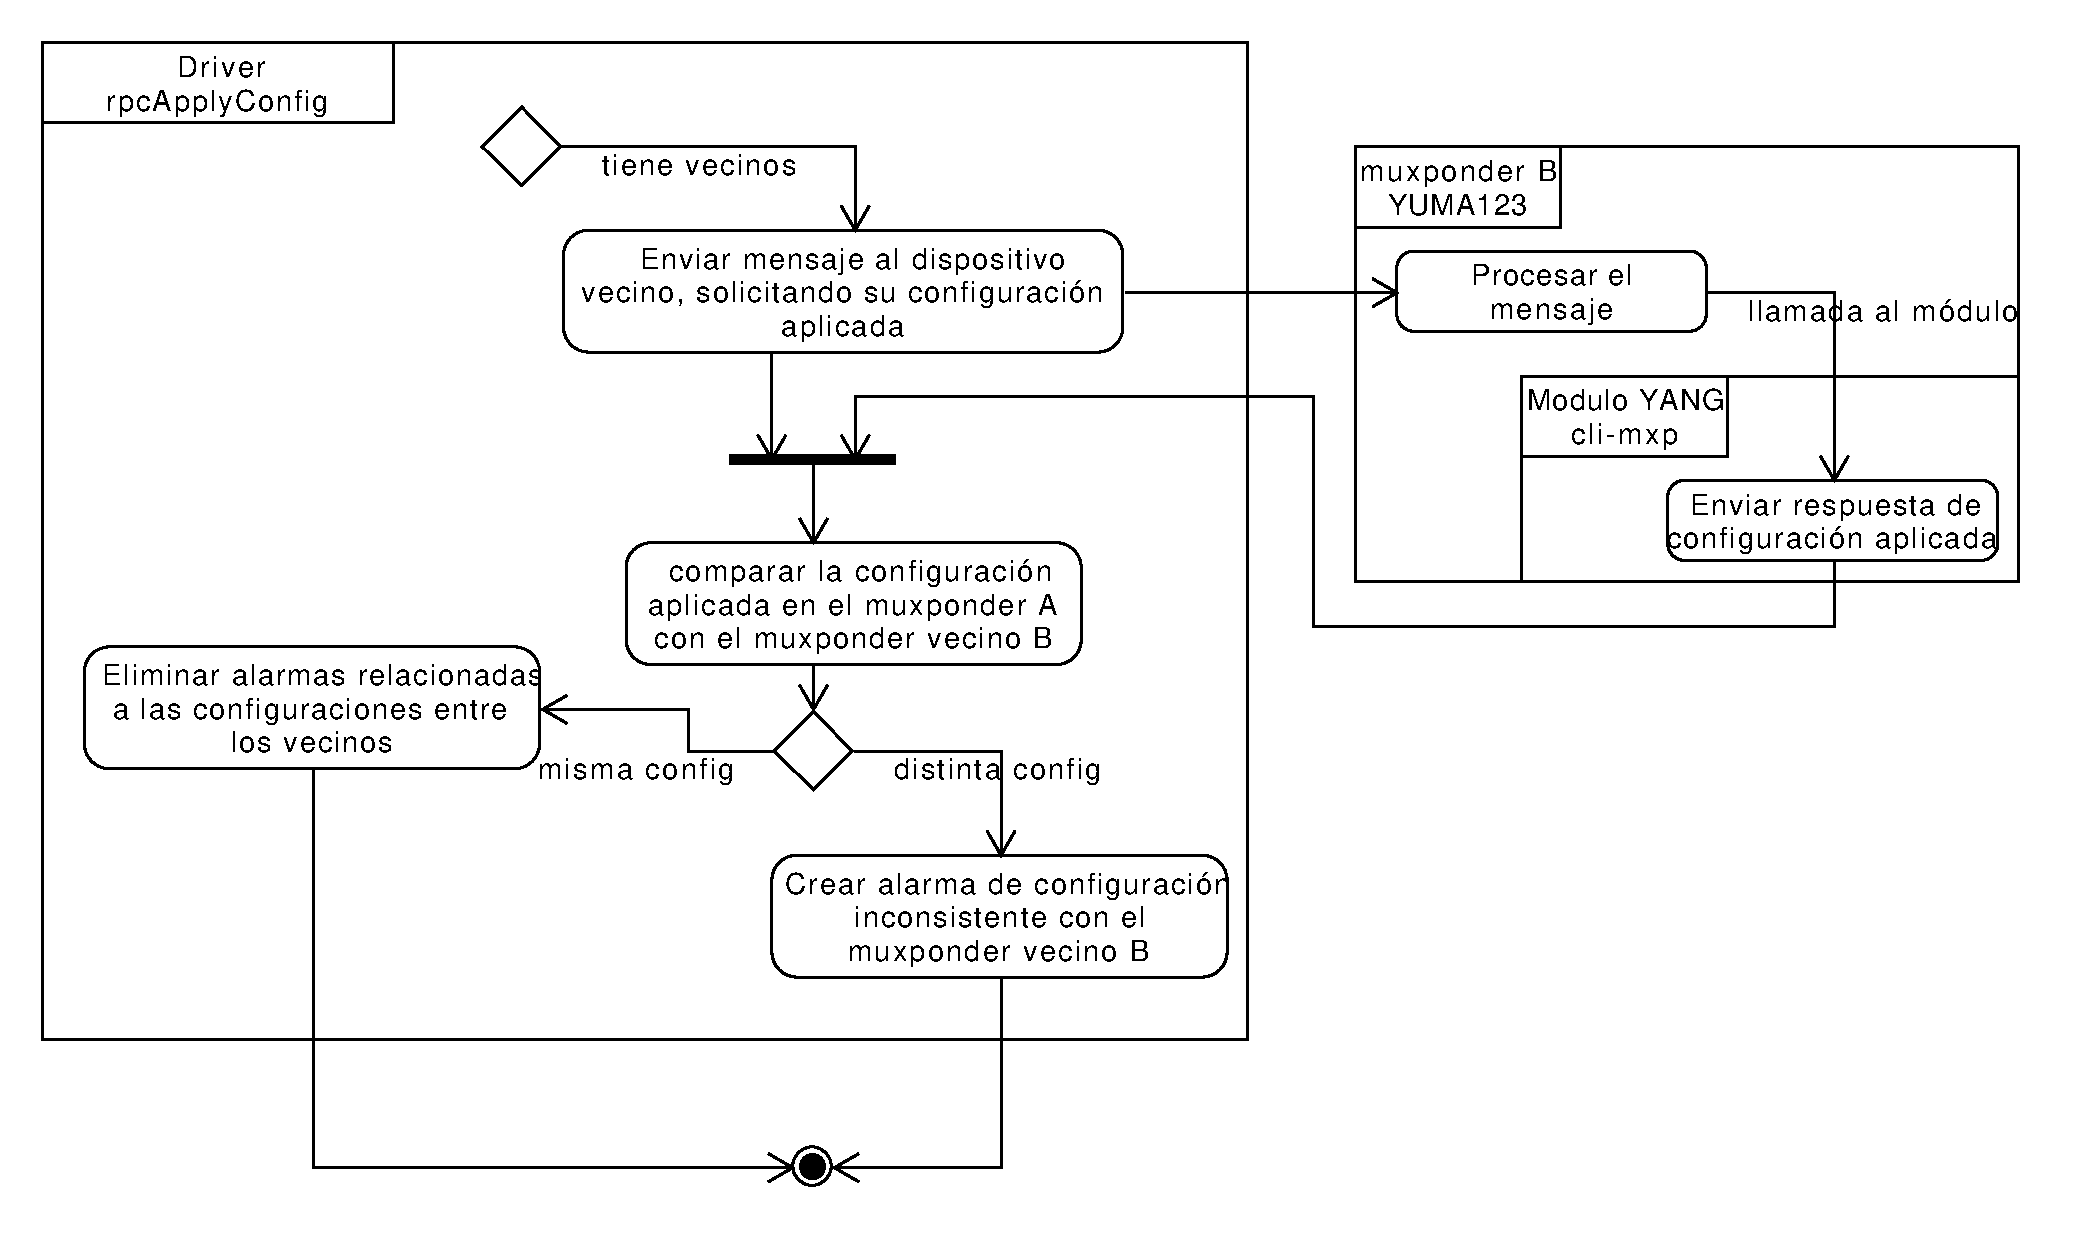
\includegraphics[scale=0.44]{Figures/actividad_driver_rpc_con_vecinos.pdf}
    \caption{Diagrama de actividad para la \textit{RPC} mux-apply-config, con vecinos.}
    \label{fig:actividad_driver_rpc_con_vecinos}
  \end{figure}

  \section{Diseño de la interfaz \textit{Northbound} e Interfaz de usuario}
  Para cumplir con los requerimientos del sistema, será necesario crear en primera instancia una interfaz \textit{REST API} a las aplicaciones externas, para que las mismas puedan comunicarse con los dispositivos administrados (\textit{muxponders}) por el controlador. Como se estudió en capítulos anteriores, \textit{ONOS} utiliza una interfaz llamada \textit{Northbound} para comunicarse con la capa de aplicación, por lo que la aplicación \textit{REST} estará ubicada en dicha interfaz. 

  También, se deberá diseñar y crear una aplicación \textit{WEB} que sirva como interfaz de usuario al administrador. A diferencia de la aplicación \textit{REST}, la \textit{GUI} desarrollada residirá en la capa de aplicación. La figura \ref{fig:ubicacionapp} esclarece la ubicación de las aplicaciones mencionadas anteriormente. 

  \begin{figure}[H]
    \centering
    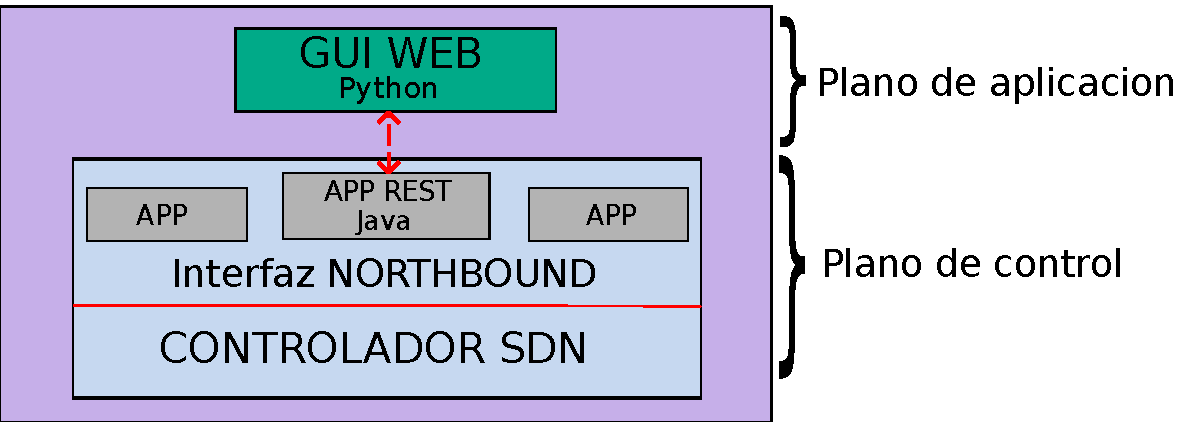
\includegraphics[scale=0.65]{Figures/arq-rest-gui.pdf}
    \caption{Interfaz \textit{REST} e interfaz de usuario.}
    \label{fig:ubicacionapp}
  \end{figure}

  \subsection{Requerimientos}

  A continuación, se listan en la figura \ref{fig:req_app} los diferentes requerimientos que deberán cumplir la interfaz \textit{REST} y la GUI. Los requerimientos R-15, R-16 y R-17 corresponden a la interfaz \textit{REST}, mientras que los requerimientos R-18 a R-21 pertenecen a la \textit{GUI} desarrollada.  

  \begin{figure}[!h]
    \centering
    \begin{subfigure}[b]{1\textwidth}
        \centering
        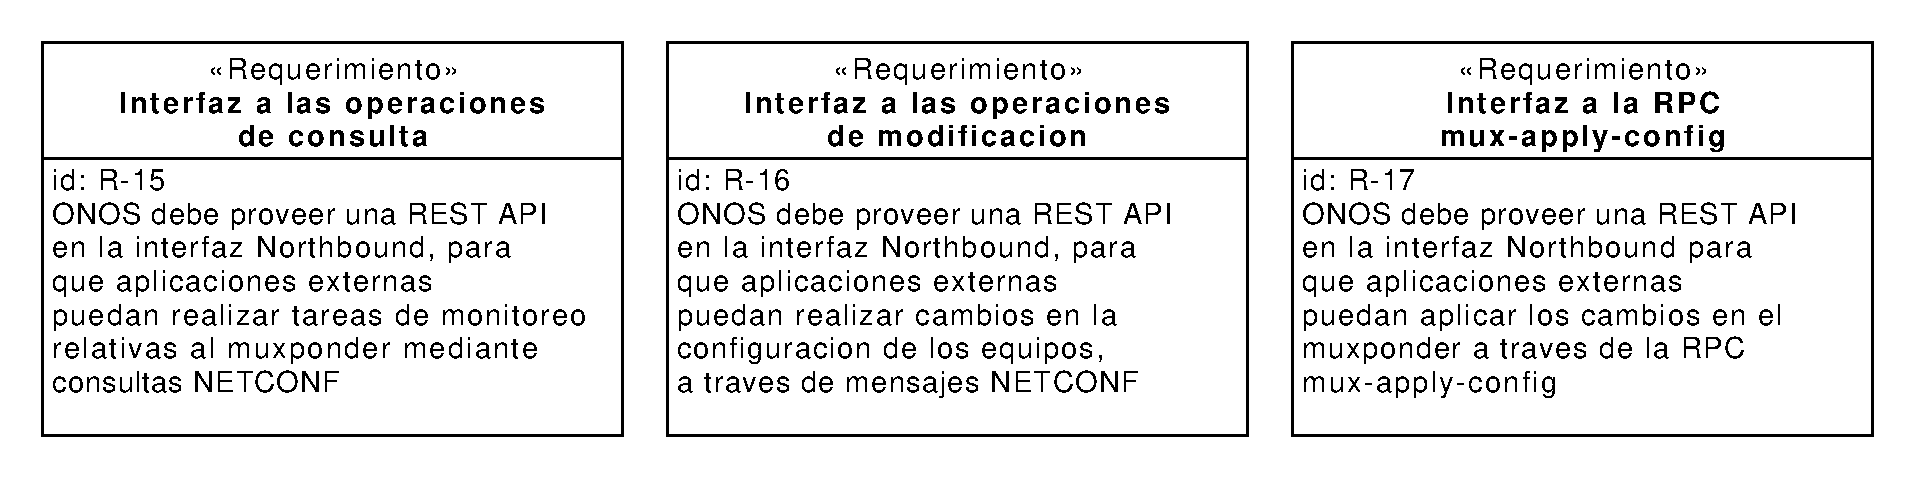
\includegraphics[width=\textwidth]{Figures/req_rest_rest.pdf}
        \caption{Requerimientos para la aplicación \textit{REST}.}
    \end{subfigure}
    \quad
    \vskip\baselineskip
    \begin{subfigure}[b]{0.75\textwidth}   
        \centering 
        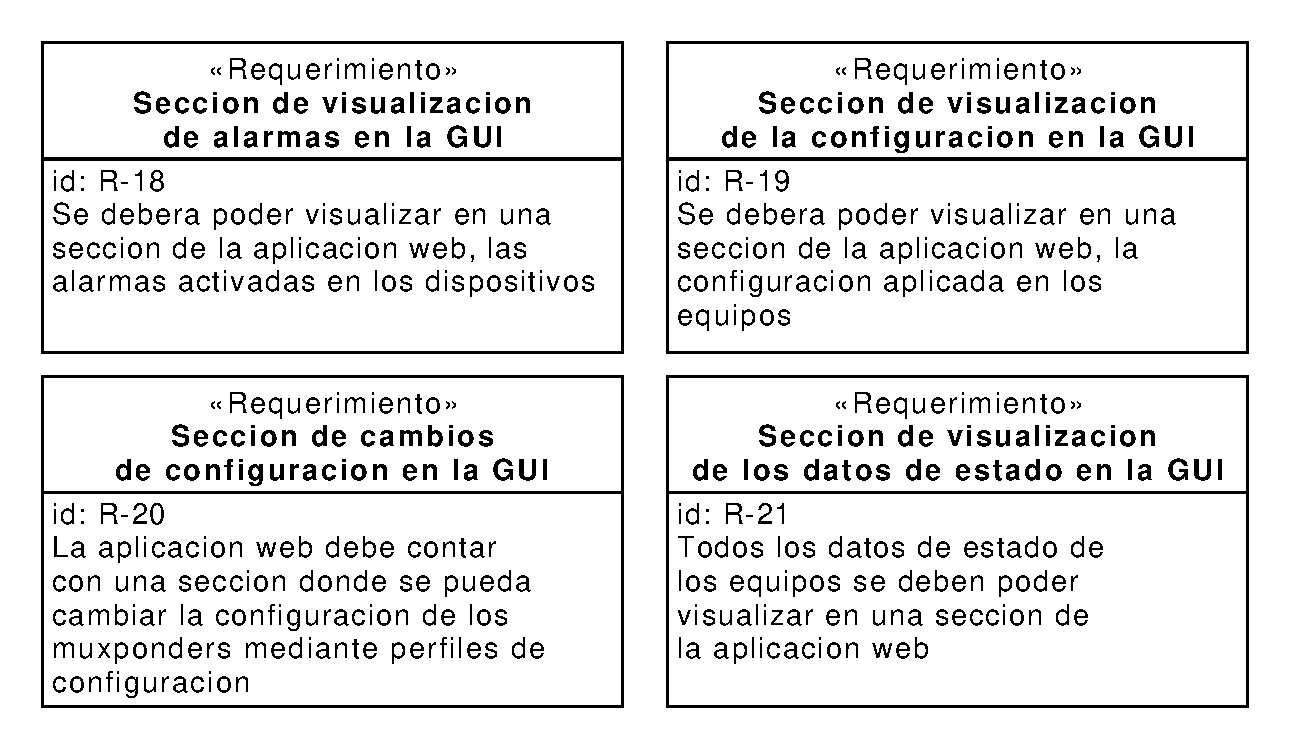
\includegraphics[width=\textwidth]{Figures/req_rest.pdf}
        \caption{Requerimientos para la aplicación \textit{WEB}.}
    \end{subfigure}
    \caption{Requerimientos.}
    \label{fig:req_app}
\end{figure}



  \subsection{Implementación de la \textit{REST}}

  Para el desarrollo de la aplicación que se ejecuta en la interfaz \textit{Northbound} del controlador, se utilizó la herramienta \textit{onos-create-app} \parencite{onosapptemplate}. La misma, crea un esqueleto de una aplicación simple con una interfaz \textit{REST}, a partir de la cual se realizaron modificaciones para poder cumplir con los requerimientos R-15, R-16 y R-17.

  Así, la aplicación \textit{REST API} se encuentra dividida en cinco clases de Java, las cuales se detallan a continuación. 


  \begin{itemize}
	\item \textbf{AppComponent}: esta clase resulta del uso de la herramienta \textit{onos-create-app}. Aquí se define el comportamiento que tendrá la aplicación al momento de su activación y desactivación. En este caso, cuando se activa la aplicación en el controlador, la misma inicia un objeto Listener para poder imprimir mensajes de log y \textit{debbug}.
    
    \item \textbf{AppWebApplication}: también resulta del uso de la aplicación mencionada anteriormente. El objetivo de esta clase, es la de indicar cuáles serán las funciones de la aplicación que se exponerán en la \textit{Northbound} interface de \textit{ONOS}.

    \item \textbf{GetWebResource}: en esta clase se definen las operaciones de consulta que son expuestas, a través de la clase AppWebApplication, a la interfaz \textit{Northbound} del controlador. En ella, se definen funciones que tienen operaciones GET de HTTP, las cuales aceptan ciertos parámetros dependiendo de la operación (por ejemplo, indicar a qué dispositivo se quiere realizar la consulta). Seguidamente, la función llama al \textit{driver} del dispositivo con los parámetros que recibió,  y devuelve una respuesta a las aplicaciones que la llamaron.
    
    \item \textbf{RpcWebResource}: de forma similar, esta clase expone una interfaz \textit{REST API} a la \textit{RPC} mux-apply-config definida en el módulo \textit{YANG}. Así, las aplicaciones externas especifican el id de un dispositivo, para que luego la interfaz \textit{REST} se comunique con el mismo mediante el \textit{driver} desarrollado. 
    
    \item \textbf{SetWebResource}: por último, se expone una interfaz con operaciones PUT de HTTP, con las cuales se posibilita que las aplicaciones externas puedan realizar cambios en las bases de datos running, candidate o startup de los dispositivos.

\end{itemize}

Se muestra en la figura \ref{fig:rest_capt} un ejemplo de la interfaz \textit{REST}. En la misma, se puede observar las diferentes operaciones expuestas explicadas anteriormente.

\begin{figure}[H]
    \centering
    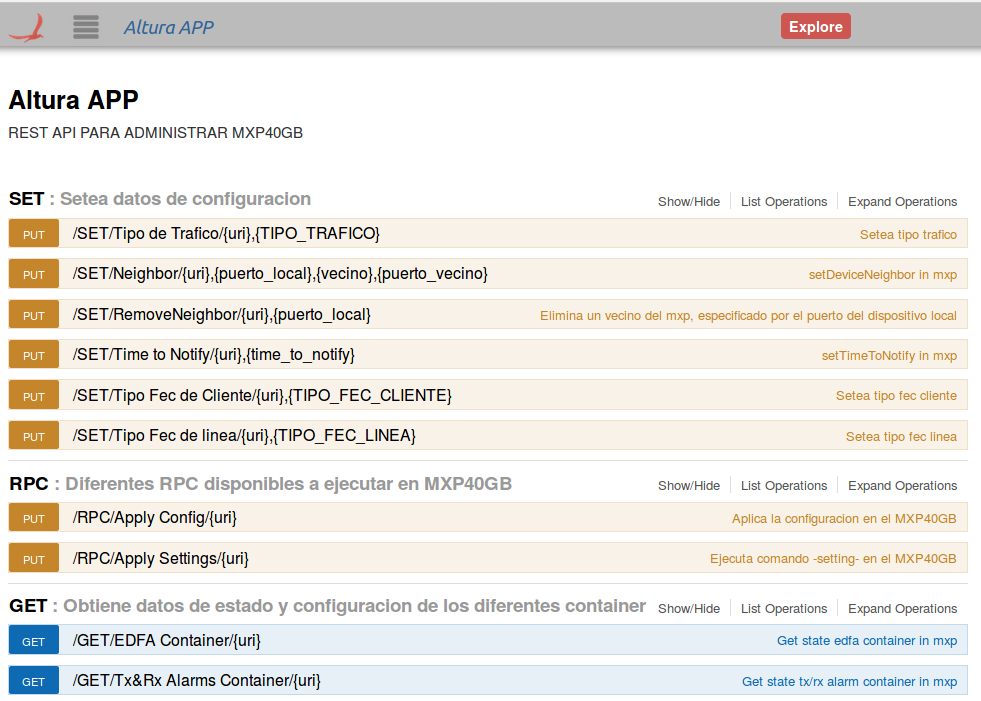
\includegraphics[scale=0.41]{Figures/captura-rest.png}
    \caption{Fragmento de la interfaz \textit{REST} implementada.}
    \label{fig:rest_capt}
  \end{figure}


  \subsection{Implementación de la interfaz de usuario}
  A fin de cumplir con los requerimientos R-18 a R-23, se realizó una aplicación \textit{WEB} basada en Flask \parencite{flask}. La misma, se desarrolla en Python y hace uso de lenguajes como HTML, JavaScript y CSS para presentar la interfaz de usuario. Cada sección listada en los requerimientos de la figura \ref{fig:req_app}, corresponde a un archivo HTML que contiene la estructura de la aplicación y los datos que se presentan en la interfaz. 

Es importante mencionar que todas las vistas realizan una tarea común. La misma consiste en consultar periódicamente al controlador, las alarmas activas que tiene \textit{ONOS} relativas a los \textit{muxponders}. Se puede observar el diagrama de actividad de la tarea mencionada en la figura \ref{fig:consulta_alarmas}.

\begin{figure}[H]
    \centering
    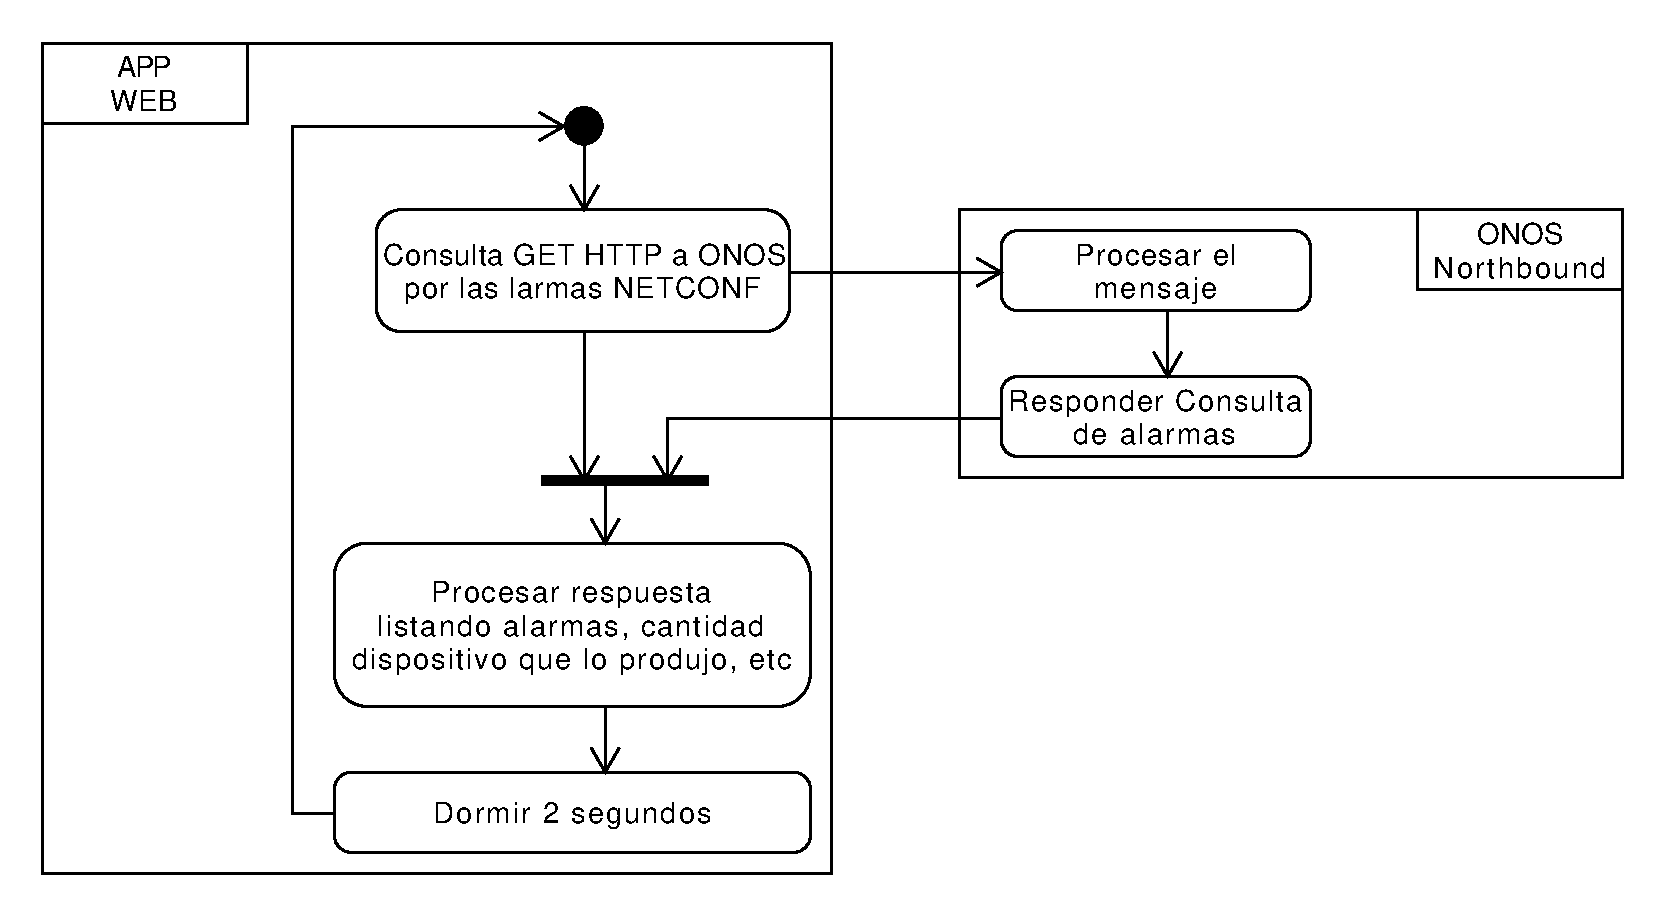
\includegraphics[scale=0.45]{Figures/consulta_alarmas.pdf}
    \caption{Consulta periódica por las alarmas al controlador \textit{ONOS}.}
    \label{fig:consulta_alarmas}
  \end{figure}

  Como ya se explicó en este capítulo, las alarmas son enviadas por los dispositivos a través de las notificaciones \textit{NETCONF}. Luego, el controlador las registra internamente, por lo que no es necesario hacer uso de la interfaz \textit{Southbound} para consultar a los equipos por el estado de las alarmas. De esta forma, los mismos se ven aliviados al no tener que procesar periódicamente estas consultas.
  \\

  Teniendo en cuenta esta actividad común, el desarrollo de la \textit{GUI} se divide en las siguientes secciones:

  \begin{itemize}
	\item \textbf{Vista principal}: muestra la cantidad de la alarmas presentes, sin entrar en detalles. A su vez, en la parte inferior de esta vista se permite agregar nuevos dispositivos a la topología, indicando la dirección IP y el puerto. Por último, en la zona superior se brinda un campo donde puede seleccionarse un conjunto de equipos para posteriormente aplicar una configuración con un perfil dado. Se puede observar en la figura \ref{fig:captura_web_principal} la interfaz gráfica que presenta esta vista.

    \begin{figure}[H]
        \centering
        \resizebox{\textwidth}{!}{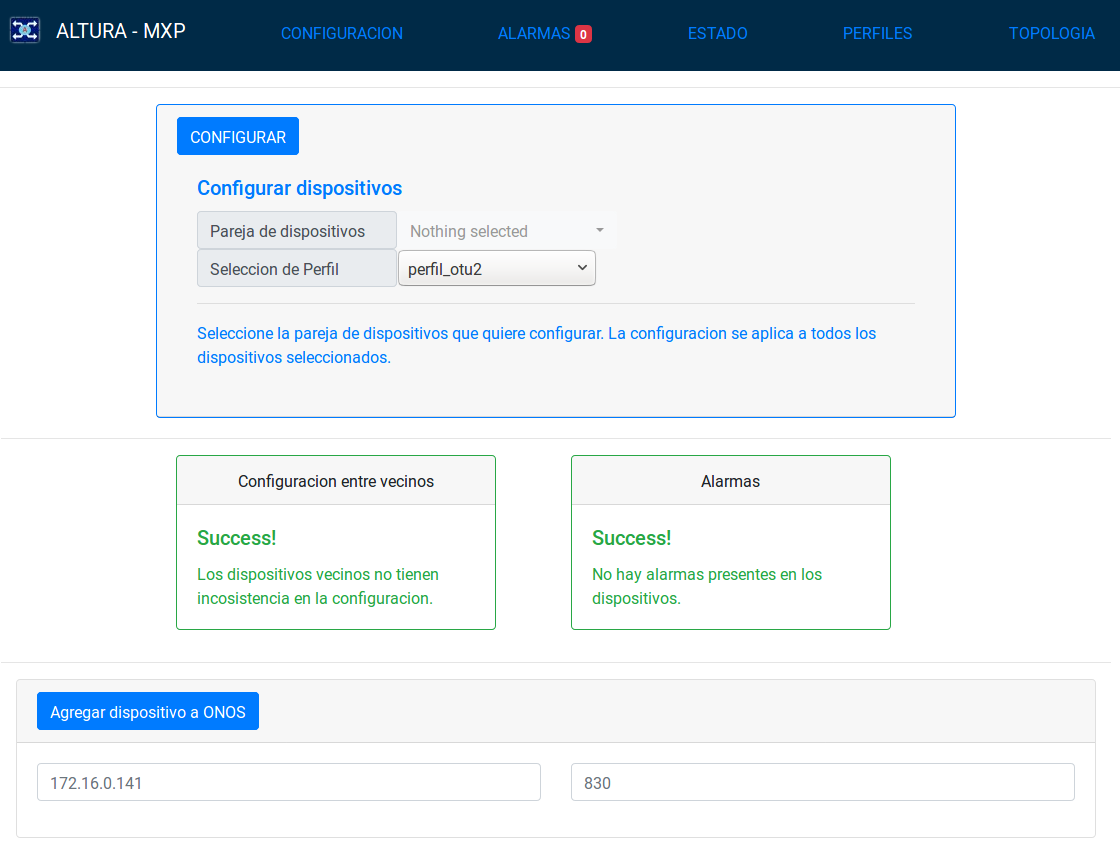
\includegraphics{Figures/vista_principal.png}}
        \caption{Interfaz de la vista principal.}
        \label{fig:captura_web_principal}
      \end{figure}

    Por otra parte, en el diagrama de la figura \ref{fig:agregar_disp_web} se muestra como la aplicación \textit{WEB} conforma un mensaje JSON con la información del equipo (dirección IP, puerto) y la envía al controlador a través de la interfaz\textit{ REST}. Luego, el controlador procesa el mensaje dando inicio al descubrimiento del dispositivo. 

    \begin{figure}[H]
        \centering
        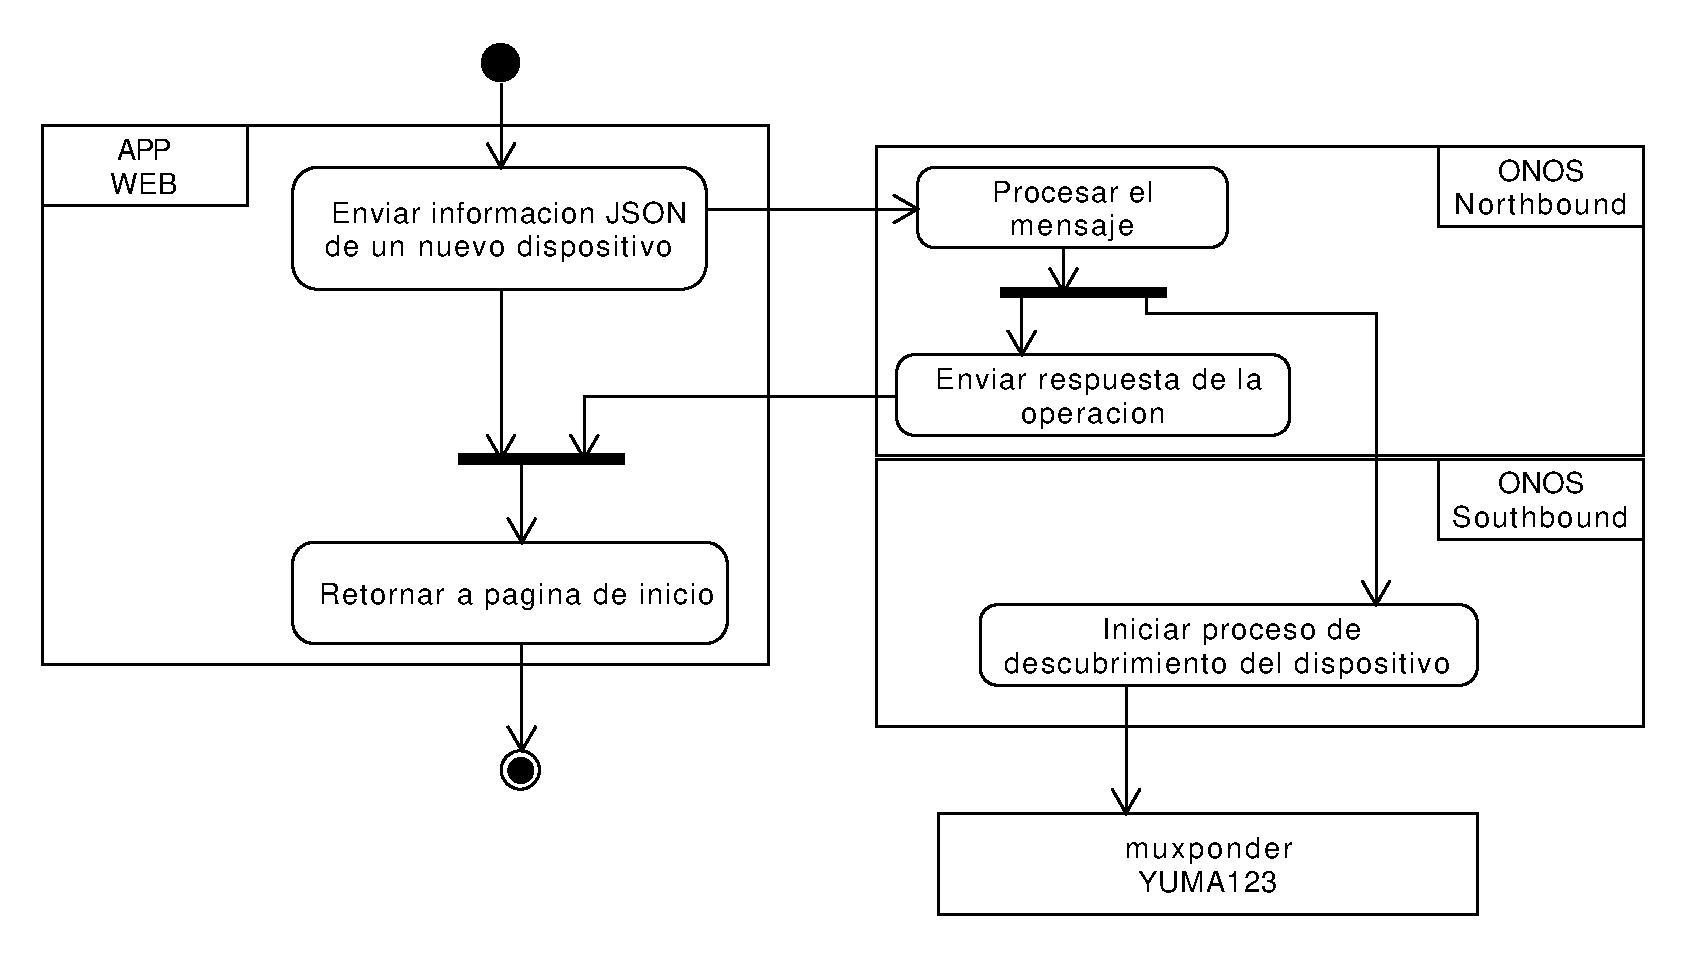
\includegraphics[scale=0.45]{Figures/agregar_disp_web.pdf}
        \caption{Agregar dispositivo a través de la APP \textit{WEB}.}
        \label{fig:agregar_disp_web}
      \end{figure}

    Por último, la figura \ref{fig:config_disp_web} muestra como es el proceso de configuración de un \textit{muxponder} a través de la GUI. Primeramente, se envia el perfil de configuración, una vez que la información es almacenada en el \textit{datastore running}, se envía la \textit{RPC} \textit{mux-apply-config} para que se apliquen los cambios en el dispositivo.

    \begin{figure}[H]
        \centering
        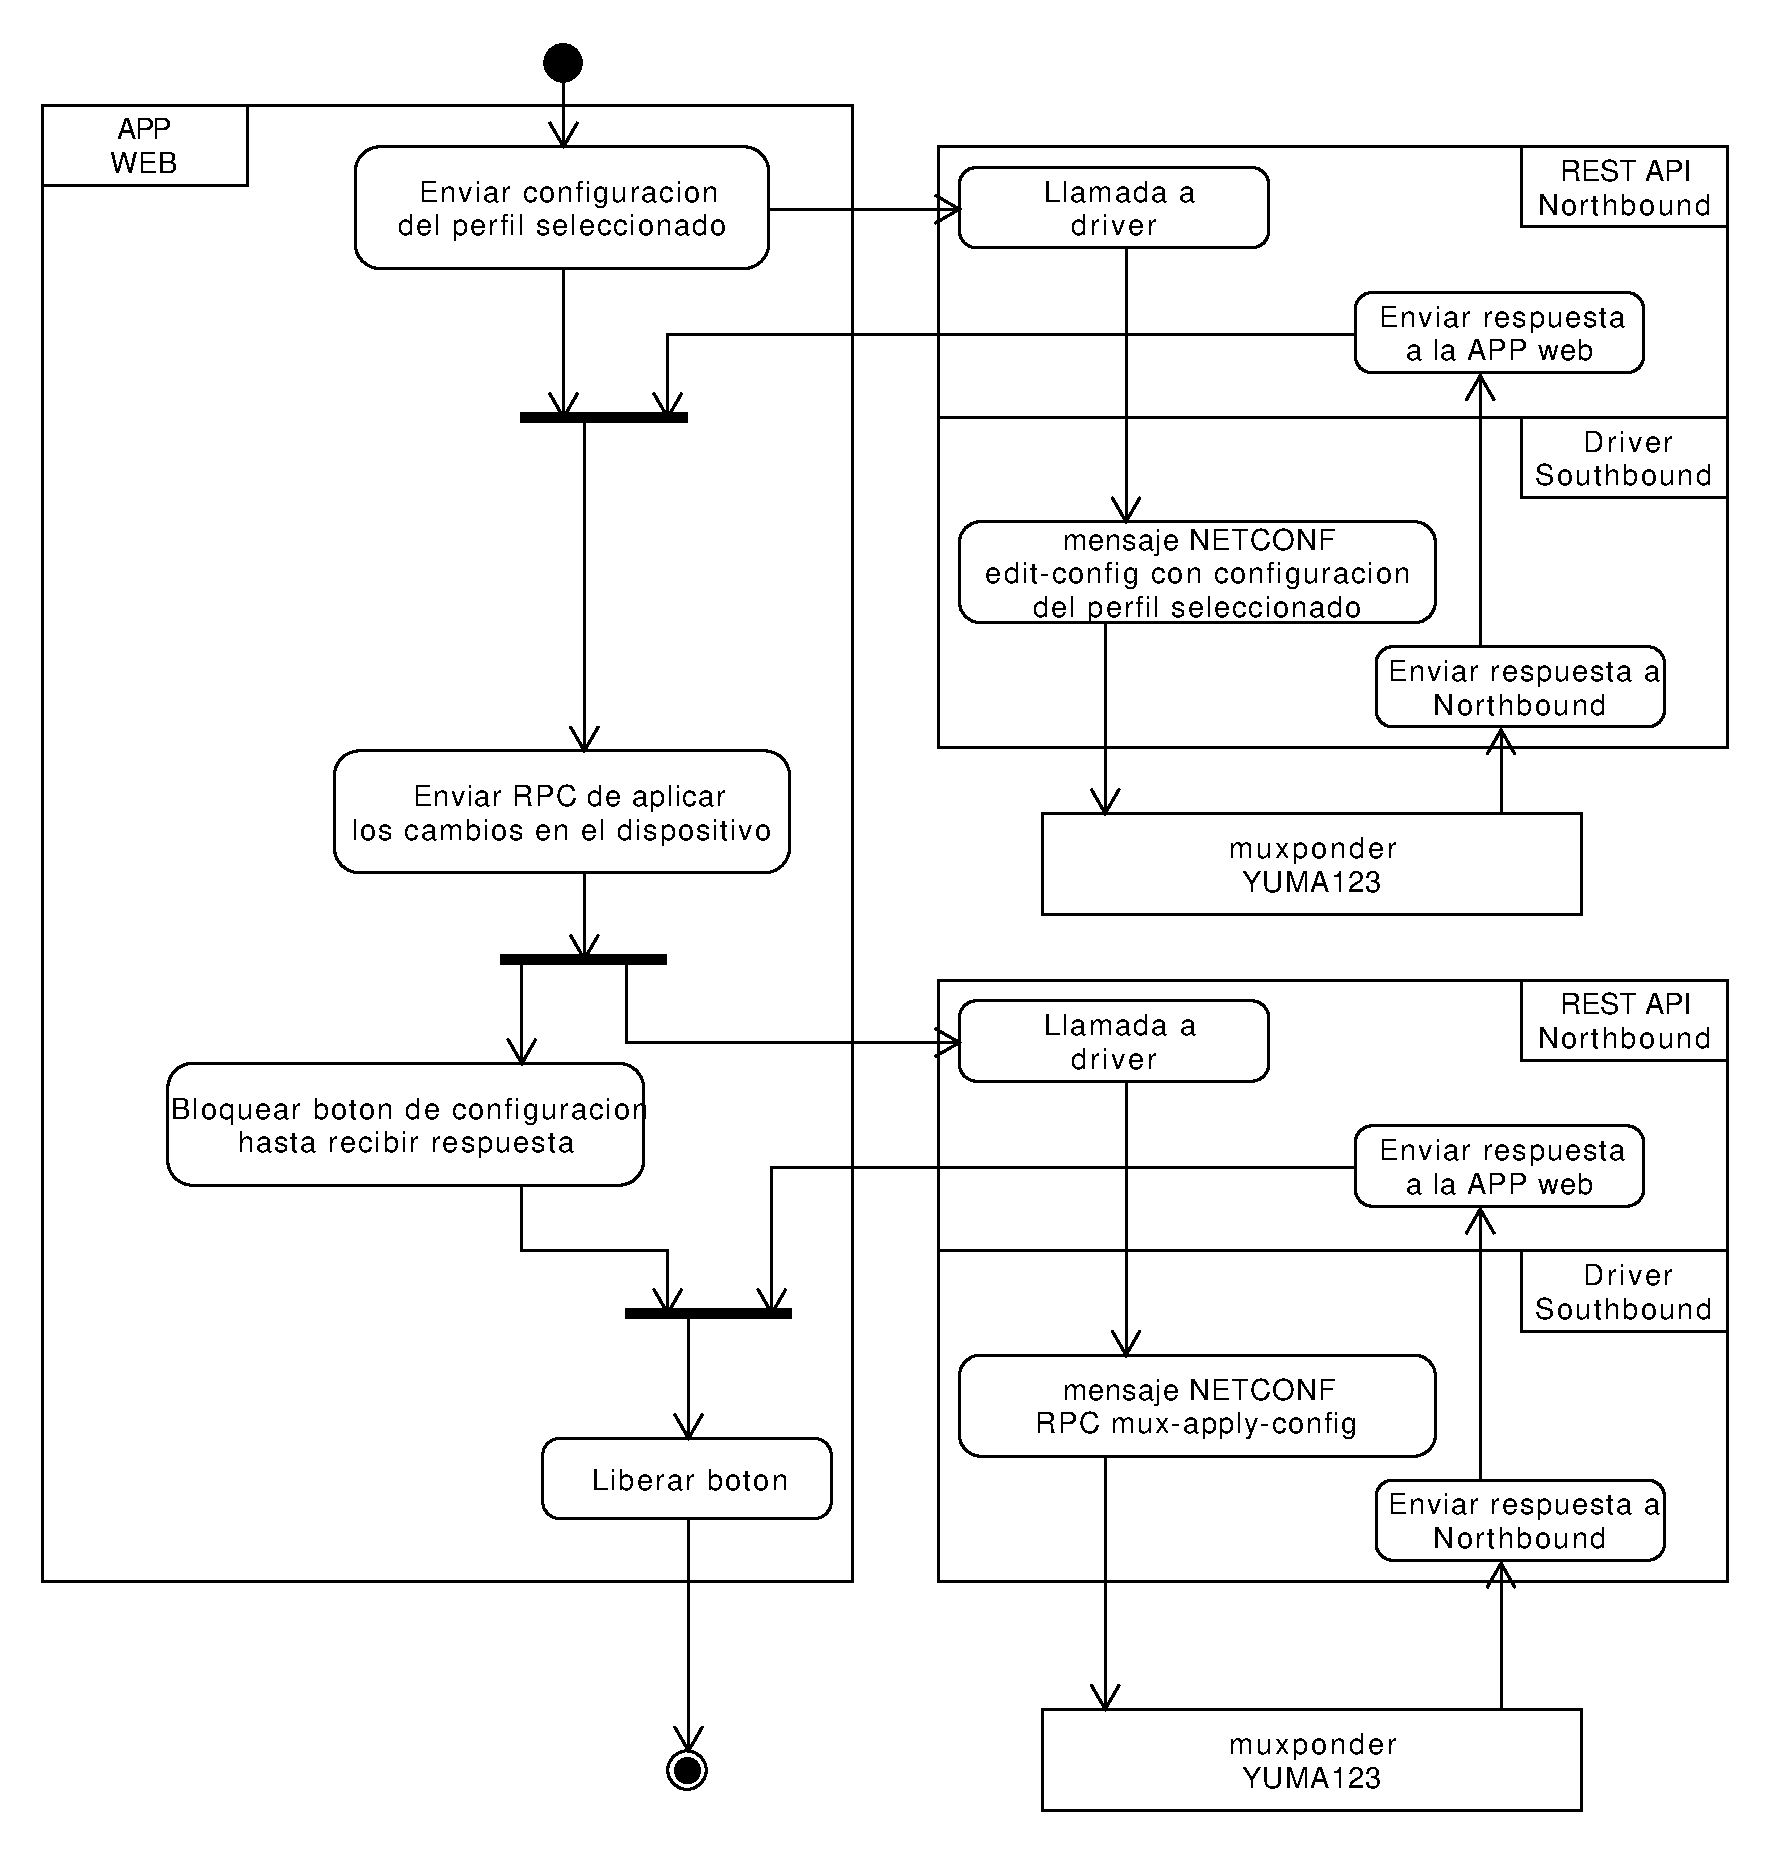
\includegraphics[scale=0.45]{Figures/config_disp_web.pdf}
        \caption{Configurar un dispositivo a través de la APP \textit{WEB}.}
        \label{fig:config_disp_web}
      \end{figure}

    \item \textbf{Vista de alarmas}: muestra una información más detallada de las alarmas. El administrador puede identificar el tipo de alarma, el dispositivo que lo originó y la cantidad de alarmas totales que presenta la topología. El diagrama de actividad que refleja el comportamiento que realiza la interfaz \textit{WEB} en esta sección, se mostró en la figura \ref{fig:consulta_alarmas}. Por otra parte, la figura \ref{fig:captura_web_alarmas} detalla el contenido de dicha sección.
   
    \begin{figure}[H]
        \centering
        \resizebox{\textwidth}{!}{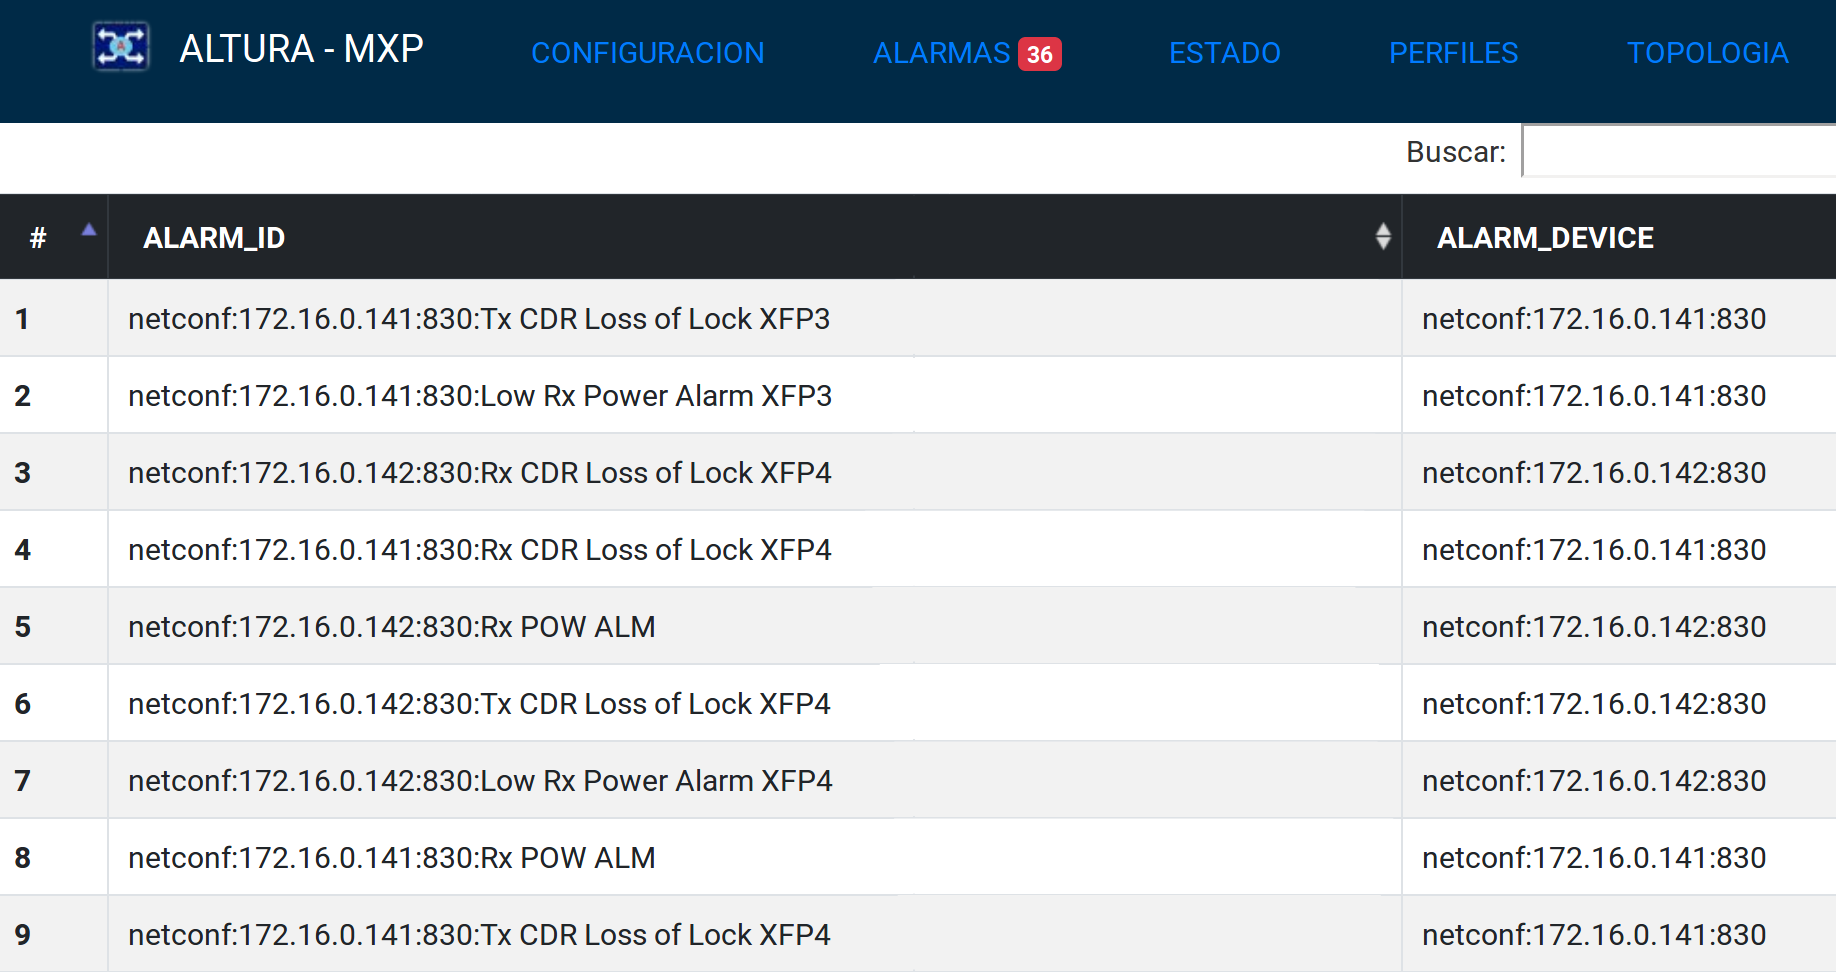
\includegraphics{Figures/vista_alarmas.png}}
        \caption{Interfaz de la vista de alarmas.}
        \label{fig:captura_web_alarmas}
      \end{figure}
    
    \item \textbf{Vista de datos de configuración}: presenta una sección donde se puede observar una lista de los equipos que conforman la topología con sus respectivas configuraciones aplicadas. La figura \ref{fig:captura_web_config} muestra esta sección. 
        
    \begin{figure}[H]
        \centering
        \resizebox{\textwidth}{!}{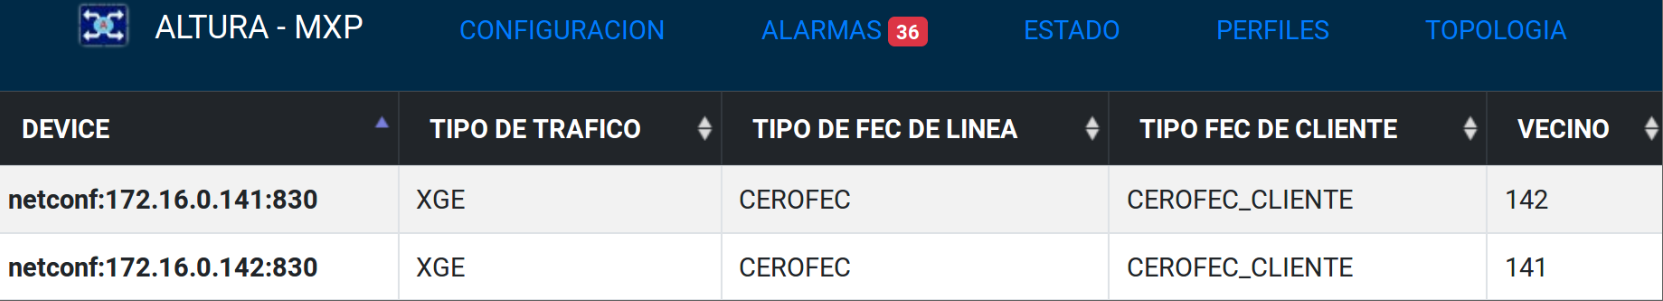
\includegraphics{Figures/vista_config.png}}
        \caption{Interfaz de la vista de configuración.}
        \label{fig:captura_web_config}
      \end{figure}

    \item \textbf{Vista de datos de estado}: de forma similar a la vista anterior, se muestra en esta sección información relacionada a los datos de estado de los equipos. A continuación, se muestra la figura \ref{fig:captura_web_estado} la interfaz que presenta esta vista, donde se puede observar en la misma los diferentes containers de estado que se implementaron en el modulo \textit{YANG}.
    
    \begin{figure}[H]
        \centering
        \resizebox{\textwidth}{!}{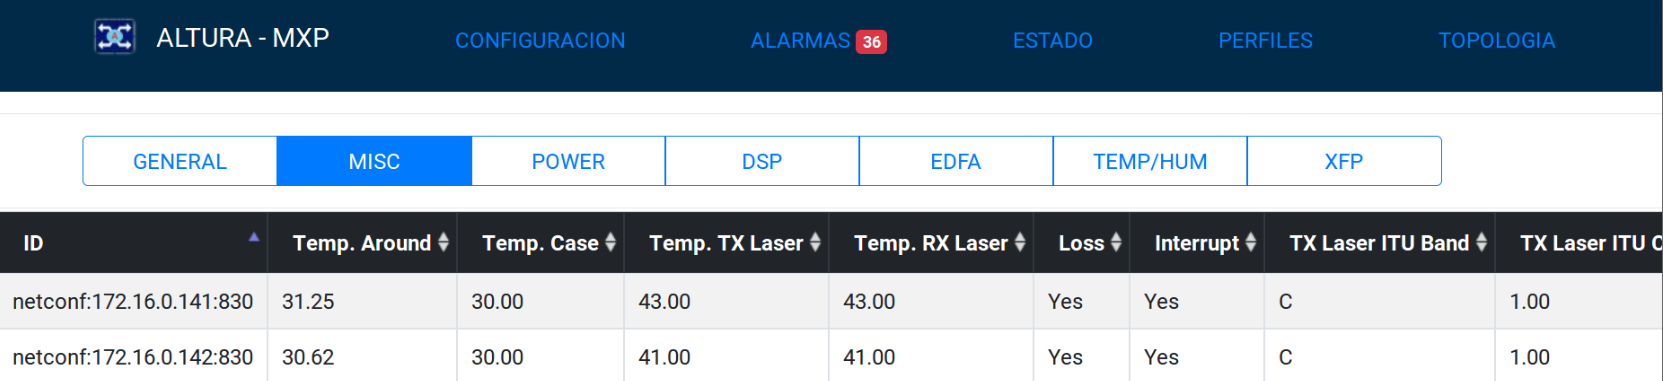
\includegraphics{Figures/vista_estado.png}}
        \caption{Interfaz de la vista de estado.}
        \label{fig:captura_web_estado}
      \end{figure}

    \item \textbf{Vista de topología}: permite realizar cambios en la topología de la red a través de mensajes \textit{NETCONF} a los dispositivos. Así, se puede especificar una pareja de equipos para que el controlador, mediante la función LinkDiscovery, pueda formar o eliminar los enlaces entre los mismos. Dicha vista se muestra en la figura \ref{fig:captura_web_topo}. 
    
    \begin{figure}[H]
        \centering
        \resizebox{\textwidth}{!}{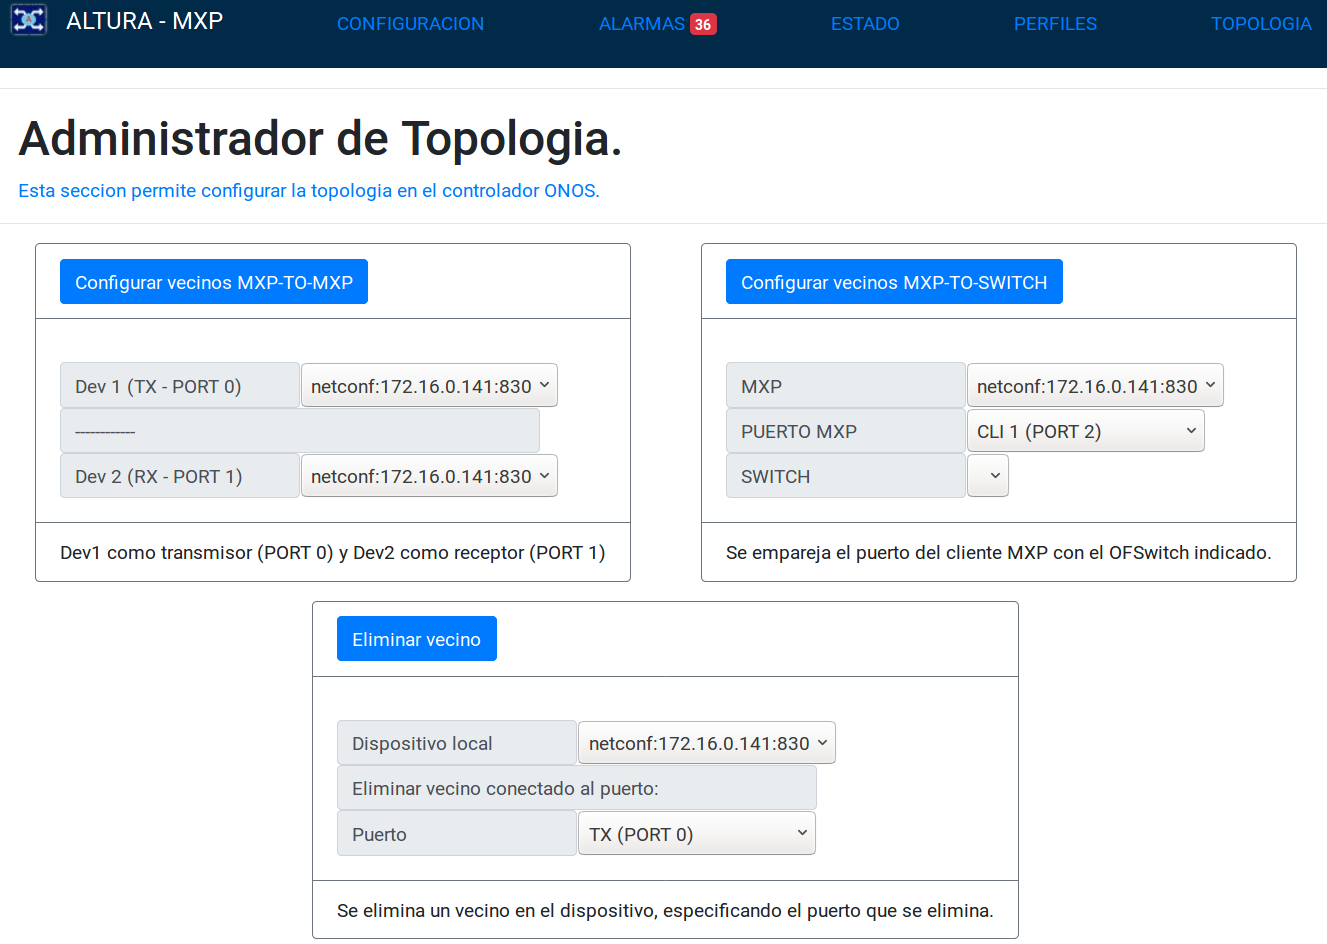
\includegraphics{Figures/vista_topo.png}}
        \caption{Interfaz de la vista de topología.}
        \label{fig:captura_web_topo}
      \end{figure}
    
    \item \textbf{Vista de perfiles}: por último, en esta vista se muestra una sección donde se permite agregar o eliminar perfiles de configuración. La idea básica de los perfiles de configuración, es la de agrupar una serie de parámetros de tal forma que el administrador pueda identificar fácilmente cuál será la configuración que se aplique en el dispositivo. Además, permite guardar dicho perfil con el fin de poder reutilizarlo en un futuro. En la figura \ref{fig:captura_web_topo}, se presenta finalmente la interfaz de esta sección.

    \begin{figure}[H]
        \centering
        \resizebox{\textwidth}{!}{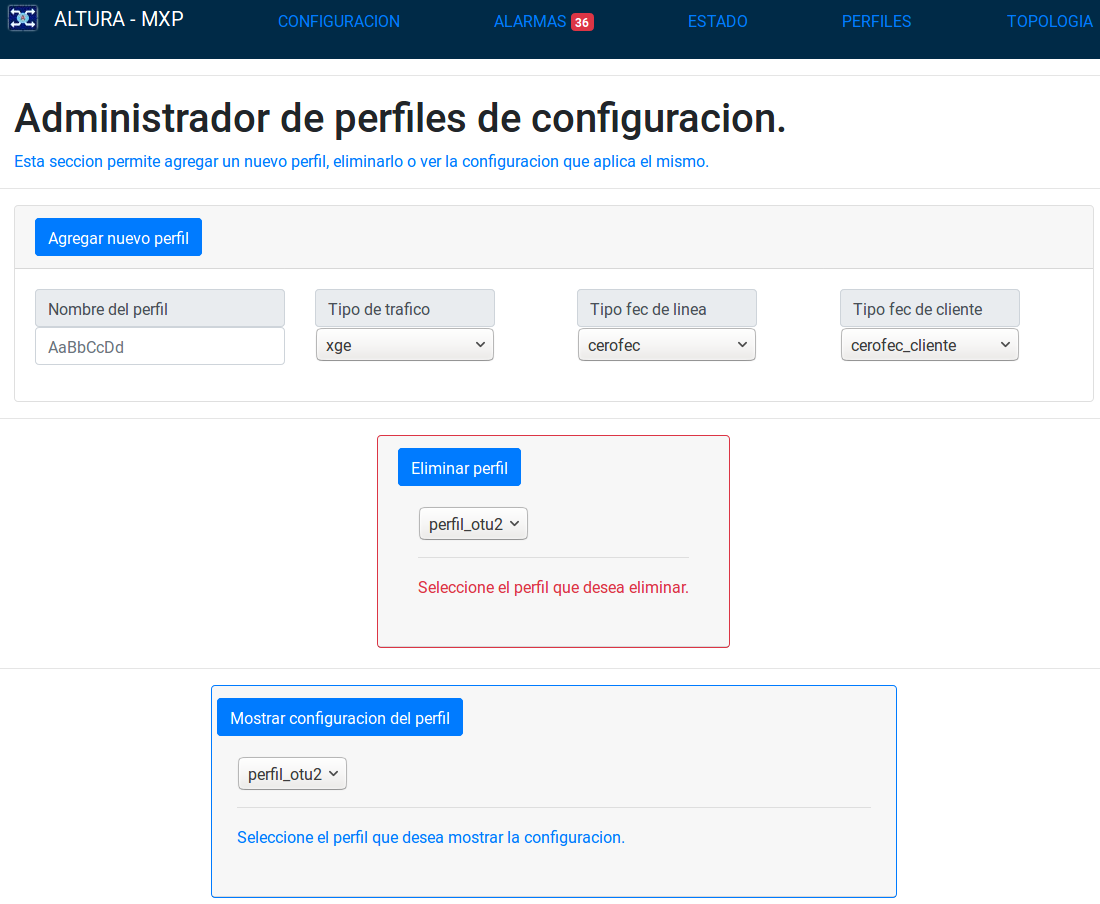
\includegraphics{Figures/vista_perfiles.png}}
        \caption{Interfaz de la vista de administración perfiles de configuración.}
        \label{fig:captura_web_topo}
      \end{figure}
    
\end{itemize}



% \subsubsection*{Casos de uso}
